\documentclass[11pt]{article}

% Upload this file to Overleaf together with the project folders
% `outputs/` and `data/` if you want the figure paths to work unchanged.

\usepackage[margin=1in]{geometry}
\usepackage{amsmath, amssymb}
\usepackage{booktabs}
\usepackage{array}
\usepackage{graphicx}
\usepackage{subcaption}
\usepackage{float}
\usepackage{xcolor}
\usepackage[round,authoryear]{natbib}
\usepackage[bookmarksnumbered]{hyperref}

\captionsetup[figure]{font=small, labelfont=small}
\captionsetup[subfigure]{font=footnotesize, labelfont=footnotesize}
\setlength{\parindent}{0pt}
\setlength{\parskip}{0.8em}
\setcounter{secnumdepth}{2}
\setcounter{tocdepth}{2}

\title{Approximate Bayesian Computation for an Adaptive-Network SIR Infection Model}
\author{
Chris Yong Hong Sen (A0257899X) \\
Eugene Xiang Yichen (A0272443H) \\
Ong Hao Yang (A0258904W)
}
\date{\today}

\begin{document}
\maketitle
\tableofcontents

\section{Introduction}

This report summarizes an Approximate Bayesian Computation (ABC) study for an adaptive-network SIR epidemic model using the scripts
\texttt{simulator.py},
\texttt{observed\_summaries.py},
\texttt{abc\_rejection.py},
\texttt{abc\_rejection\_regression.py}, and
\texttt{abc\_mcmc.py}, and
\texttt{smc\_abc.py}.
We consider an SIR epidemic evolving on an adaptive contact network with $N = 200$ agents. The network changes dynamically because susceptible individuals may rewire connections away from infected neighbors, so disease transmission and network topology are coupled rather than treated as separate mechanisms.

The inferential target is the posterior distribution of the three model parameters
\[
\theta = (\beta,\gamma,\rho),
\]
where $\beta$ is the transmission probability, $\gamma$ is the recovery probability, and $\rho$ is the rewiring probability. Our goal is to infer these parameters from observed epidemic trajectories across $R = 40$ independent replicates.

The likelihood of the observed data given $\theta$ is intractable. Even a single epidemic trajectory depends on the joint probability of many correlated infection, recovery, and rewiring events occurring over time on an evolving random graph. The contact network itself is a high-dimensional latent object, and inference would require marginalizing over an enormous collection of possible network histories that are never directly observed. In practice, this makes direct likelihood-based methods such as maximum likelihood estimation or standard conjugate Bayesian analysis infeasible.

This motivates simulation-based inference, which bypasses explicit likelihood evaluation by comparing features of simulated and observed data. In this project the chosen SBI method is ABC, where simulated epidemics are accepted when their summary statistics are sufficiently close to the observed summary statistics. The advanced methods studied beyond basic rejection ABC are regression adjustment \citep{beaumont2002}, ABC-MCMC \citep{marjoram2003}, and SMC-ABC.

The simulator in \texttt{simulator.py} uses an adaptive contact network with an Erd\H{o}s--R\'enyi initial graph of edge probability $p_{\text{edge}}=0.05$, $5$ initially infected individuals, and a horizon of $T=200$ discrete time steps. At each step the model applies infection, recovery, and network rewiring, so the network co-evolves with the epidemic throughout the simulation.

The script \texttt{observed\_summaries.py} aggregates $40$ observed replicates into eight summary statistics, which are then matched against simulated summaries inside the ABC procedures. Details regarding the choice of summary statistics are provided in Table~\ref{tab:summary-statistics-role}. The observed summaries used in this run are listed in Table~\ref{tab:observed-summaries}.

\begin{table}[H]
\centering
\caption{Observed summary statistics computed by \texttt{observed\_summaries.py}.}
\label{tab:observed-summaries}
\begin{tabular}{>{\raggedright\arraybackslash}p{0.62\textwidth}r}
\toprule
Summary statistic & Observed value \\
\midrule
Max infection fraction & 0.657125 \\
Time to peak & 8.750000 \\
Early growth rate of infection & 0.372293 \\
Early growth rate of rewiring & 0.171150 \\
Variance structure of degree counts & 10.341023 \\
Late decay rate of infection & -0.083322 \\
Rewiring per infection & 48.093619 \\
Infection peak width at half maximum & 12.450000 \\
\bottomrule
\end{tabular}
\end{table}

More precisely, let $Y^{(r)}$ denote the data from replicate $r \in \{1,\dots,R\}$, and let $\eta_j(\cdot)$ denote the $j$th replicate-level summary functional. The implementation first computes the summary within each replicate and then averages across replicates, so the observed summary fed into ABC is
\[
\widehat{s}^{\,\mathrm{obs}}_j
= \frac{1}{R}\sum_{r=1}^{R} \eta_j\!\left(Y^{(r)}\right),
\qquad j=1,\dots,8.
\]
In statistical terms, $\widehat{s}^{\,\mathrm{obs}}_j$ is the empirical mean of the replicate-level summaries and is used as an estimator of the population quantity
\[
s_j^{\mathrm{obs}} = \mathbb{E}\!\left[\eta_j(Y)\right].
\]
Under the assumption that the $R=40$ observed replicates are independent realizations from the same underlying epidemic mechanism, the sample average above is a natural estimator of this expectation and converges to $\mathbb{E}[\eta_j(Y)]$ by the law of large numbers.

This is exactly how \texttt{observed\_summaries.py} is written. For example, the observed maximum infection fraction is computed as
\[
\widehat{s}^{\,\mathrm{obs}}_1
= \frac{1}{R}\sum_{r=1}^{R} \max_t I_t^{(r)},
\]
the observed time to peak is
\[
\widehat{s}^{\,\mathrm{obs}}_2
= \frac{1}{R}\sum_{r=1}^{R} \arg\max_t I_t^{(r)},
\]
and the same averaging principle is applied to the early-growth slopes, rewiring slopes, per-replicate degree variances, late-decay slopes, rewiring-per-infection ratios, and peak widths at half maximum. Hence the values in Table~\ref{tab:observed-summaries} should be interpreted as empirical approximations to expected summary statistics, rather than as summaries from a single trajectory.

The ABC workflow follows a standard simulation-based inference pattern. Parameter draws are sampled from the priors
\[
\beta \sim \mathrm{Unif}(0.05,0.50), \qquad
\gamma \sim \mathrm{Unif}(0.02,0.20), \qquad
\rho \sim \mathrm{Unif}(0,0.80),
\]
the epidemic is simulated, the eight summaries are computed, and the simulated summaries are compared with the observed summaries after standardization. This report first analyzes the basic ABC rejection results, then studies three extensions that move beyond the raw rejection posterior: regression adjustment, ABC-MCMC, and SMC-ABC.
\section{Basic ABC Rejection}

\subsection{Algorithm}

The baseline algorithm is implemented in \texttt{abc\_rejection.py}. It follows the standard rejection-ABC logic of simulating from the prior and retaining draws whose summaries lie close to the observed summaries \citep{beaumont2002}. The current script performs $N_{\text{sim}}=100{,}000$ prior simulations and stores the simulated parameter vector and corresponding eight-dimensional summary vector from each run. Because the summaries are on very different scales, the script standardizes them using the simulation mean and standard deviation before computing distances. If $s_i$ denotes the simulated summary vector and $s_{\text{obs}}$ denotes the observed summary vector, then the distance used in the script is
\[
d_i = \left\lVert \tilde{s}_i - \tilde{s}_{\text{obs}} \right\rVert_2,
\]
where tildes indicate the simulation-based standardization.

Implementation-wise, \texttt{abc\_rejection.py} generates independent prior draws, simulates the epidemic and rewiring trajectories, computes the eight summaries
\[
(s_1,\ldots,s_8),
\]
standardizes those summaries relative to the simulated reference bank, and then accepts the simulations whose Euclidean distances from the observed summary vector fall below the relevant empirical distance quantile. The same saved simulation bank is then reused for the reduced-set study A--I, and the final Reduced set I calibration is exported to \texttt{data/intermediate/abc\_rejection\_output.npz} for all downstream methods.

For a chosen acceptance proportion $\epsilon$, the rejection sampler sets the tolerance to the empirical $\epsilon$-quantile of the simulated distances. Equivalently, a draw is accepted if
\[
d_i \le q_{\epsilon},
\]
where $q_{\epsilon}$ is the empirical quantile of the distance distribution. This is a convenient way to control the posterior sample size directly. In the present run, the script experiments with
\[
\epsilon \in \{0.005,\; 0.01,\; 0.03\},
\]
so the accepted sample sizes are exactly $500$, $1000$, and $3000$ respectively.

The eight summaries were chosen to cover both epidemic shape and network adaptation. Their roles in the inference procedure are summarized in Table~\ref{tab:summary-statistics-role}.

\begin{table}[H]
\centering
\caption{Summary statistics used in the ABC procedures. The descriptions match the implementation in \texttt{abc\_rejection.py} and \texttt{observed\_summaries.py}.}
\label{tab:summary-statistics-role}
\begin{tabular}{>{\raggedright\arraybackslash}p{0.28\textwidth} >{\raggedright\arraybackslash}p{0.16\textwidth} >{\raggedright\arraybackslash}p{0.46\textwidth}}
\toprule
Summary statistic & Parameter informed & Notes \\
\midrule
Max infection fraction & $\beta$ & Captures overall outbreak size. In the implementation this is the maximum of the simulated infected-fraction trajectory. \\
Time to peak & $\beta, \gamma$ & Captures how quickly the epidemic reaches its maximum. In the script this is the index of the peak infected fraction. \\
Early growth rate of infection & $\beta, \gamma$ & Computed as the linear slope of $\log(I_t)$ over the early window $t=2,\dots,6$. This targets the initial expansion phase of the epidemic. \\
Early growth rate of rewiring & mostly $\rho$ & Computed as the linear slope of $\log(W_t)$ over $t=2,\dots,6$. This measures how strongly rewiring activity builds up early in the outbreak. \\
Variance structure of degree counts & $\rho$ & Computed from the final degree histogram. Higher rewiring changes the network away from the initial Erd\H{o}s--R\'enyi degree structure, so this summary is informative about network adaptation. \\
Late decay rate of infection & $\gamma, \rho$ & Computed as the linear slope of $\log(I_t)$ over the late window $t=13,\dots,20$. This captures how quickly infection declines once recovery and rewiring effects have accumulated. \\
Rewiring per infection & $\rho$ & Defined as total rewiring activity divided by total infection burden over the trajectory. This normalizes rewiring intensity by epidemic size. \\
Infection peak width at half maximum & $\beta, \gamma$ & Defined as the duration for which $I_t$ remains above half of its peak value. This captures the temporal breadth of the epidemic peak. \\
\bottomrule
\end{tabular}
\end{table}

Taken together, the summaries combine early epidemic-shape information from maximum infection, time to peak, early infection growth, and peak width with network-adaptation information from early rewiring growth, degree variance, and rewiring per infection, while the late-decay summary captures how infection dies out after recovery and rewiring have both had time to act.

\subsection{Epsilon Experimentation}

The tolerance experiment in \texttt{abc\_rejection.py} compares the posterior under the three acceptance levels above. The main body focuses on the two critical conclusions. First, the posterior center is reasonably stable across the three tolerances, so the broad posterior location is not being determined by one arbitrary cutoff. Second, the posterior widens as $\epsilon$ is relaxed, especially in the upper tails of $\beta$ and $\rho$, which is the expected bias--variance trade-off in rejection ABC. The detailed summary-by-summary overlay discussion is deferred to Appendix~\ref{app:rejection-diagnostics}.

\begin{table}[H]
\centering
\caption{Rich-set ABC rejection posterior summaries from the saved CSV outputs in \texttt{outputs/basic\_abc/param\_estimates/}. Intervals are empirical 95\% posterior intervals.}
\label{tab:epsilon-results}
\begin{tabular}{cccc}
\toprule
$\epsilon$ & Parameter & Posterior mean & 95\% interval \\
\midrule
0.005 & $\beta$ & 0.1687 & [0.1044,\ 0.2481] \\
0.005 & $\gamma$ & 0.0828 & [0.0608,\ 0.1097] \\
0.005 & $\rho$ & 0.3174 & [0.1420,\ 0.4973] \\
\midrule
0.010 & $\beta$ & 0.1733 & [0.1070,\ 0.2679] \\
0.010 & $\gamma$ & 0.0846 & [0.0595,\ 0.1152] \\
0.010 & $\rho$ & 0.3131 & [0.1065,\ 0.5402] \\
\midrule
0.030 & $\beta$ & 0.1852 & [0.1034,\ 0.3055] \\
0.030 & $\gamma$ & 0.0874 & [0.0565,\ 0.1275] \\
0.030 & $\rho$ & 0.3136 & [0.0578,\ 0.6117] \\
\bottomrule
\end{tabular}
\end{table}

These results support $\epsilon=0.01$ as the basic-ABC working tolerance. Relative to $\epsilon=0.005$, it doubles the accepted sample size from $500$ to $1000$ and therefore reduces Monte Carlo roughness. Relative to $\epsilon=0.03$, it maintains a visibly tighter posterior, especially in the right tails of $\beta$ and $\rho$. This is the tolerance later exported as the reference calibration for all downstream extensions.

\subsection{Summary Statistics Experimentation}

The next question is whether all eight summaries are needed. The same script, \texttt{abc\_rejection.py}, compares the full ``Rich set'' against reduced subsets A--I. In the current version of the project, the main selection evidence comes from two complementary diagnostics saved under \texttt{outputs/basic\_abc/summary\_set\_study/}: posterior-comparison plots against the rich set and a heatmap of normalized posterior spread. The reduced sets defined in the script are summarized in Table~\ref{tab:reduced-sets}.

\begin{table}[H]
\centering
\caption{Reduced summary-statistic sets studied in \texttt{abc\_rejection.py}.}
\label{tab:reduced-sets}
\begin{tabular}{>{\raggedright\arraybackslash}p{0.18\textwidth} >{\raggedright\arraybackslash}p{0.72\textwidth}}
\toprule
Summary set & Included summaries \\
\midrule
Reduced set A & max infection, time to peak, early infection growth, late infection decay \\
Reduced set B & max infection, time to peak, early infection growth, late infection decay, early rewiring growth \\
Reduced set C & early infection growth, late infection decay, early rewiring growth, degree variance \\
Reduced set D & max infection, late infection decay, early rewiring growth, degree variance \\
Reduced set E & max infection, time to peak, late infection decay, early rewiring growth, degree variance \\
Reduced set F & max infection, early infection growth, early rewiring growth, degree variance \\
Reduced set G & max infection, time to peak, late infection decay, early rewiring growth, degree variance, rewiring per infection \\
Reduced set H & max infection, time to peak, early rewiring growth, degree variance, rewiring per infection \\
Reduced set I & max infection, time to peak, early rewiring growth, degree variance, rewiring per infection, peak width at half maximum \\
\bottomrule
\end{tabular}
\end{table}

Figure~\ref{fig:summary-set-selection} isolates the critical evidence used in the final choice. The left panel compares the rich-set posterior with Reduced set I at $\epsilon=0.01$, while the right panel shows the posterior-spread heatmap. Numerically, the rich-set posterior means at $\epsilon=0.01$ are
\[
(\mathbb{E}[\beta],\mathbb{E}[\gamma],\mathbb{E}[\rho]) = (0.1733,\ 0.0846,\ 0.3131),
\]
whereas the corresponding Reduced set I means are
\[
(0.1730,\ 0.0844,\ 0.3109).
\]
These differences are negligible for the purposes of this analysis.

\begin{figure}[H]
\centering
\begin{subfigure}[t]{0.48\textwidth}
    \centering
    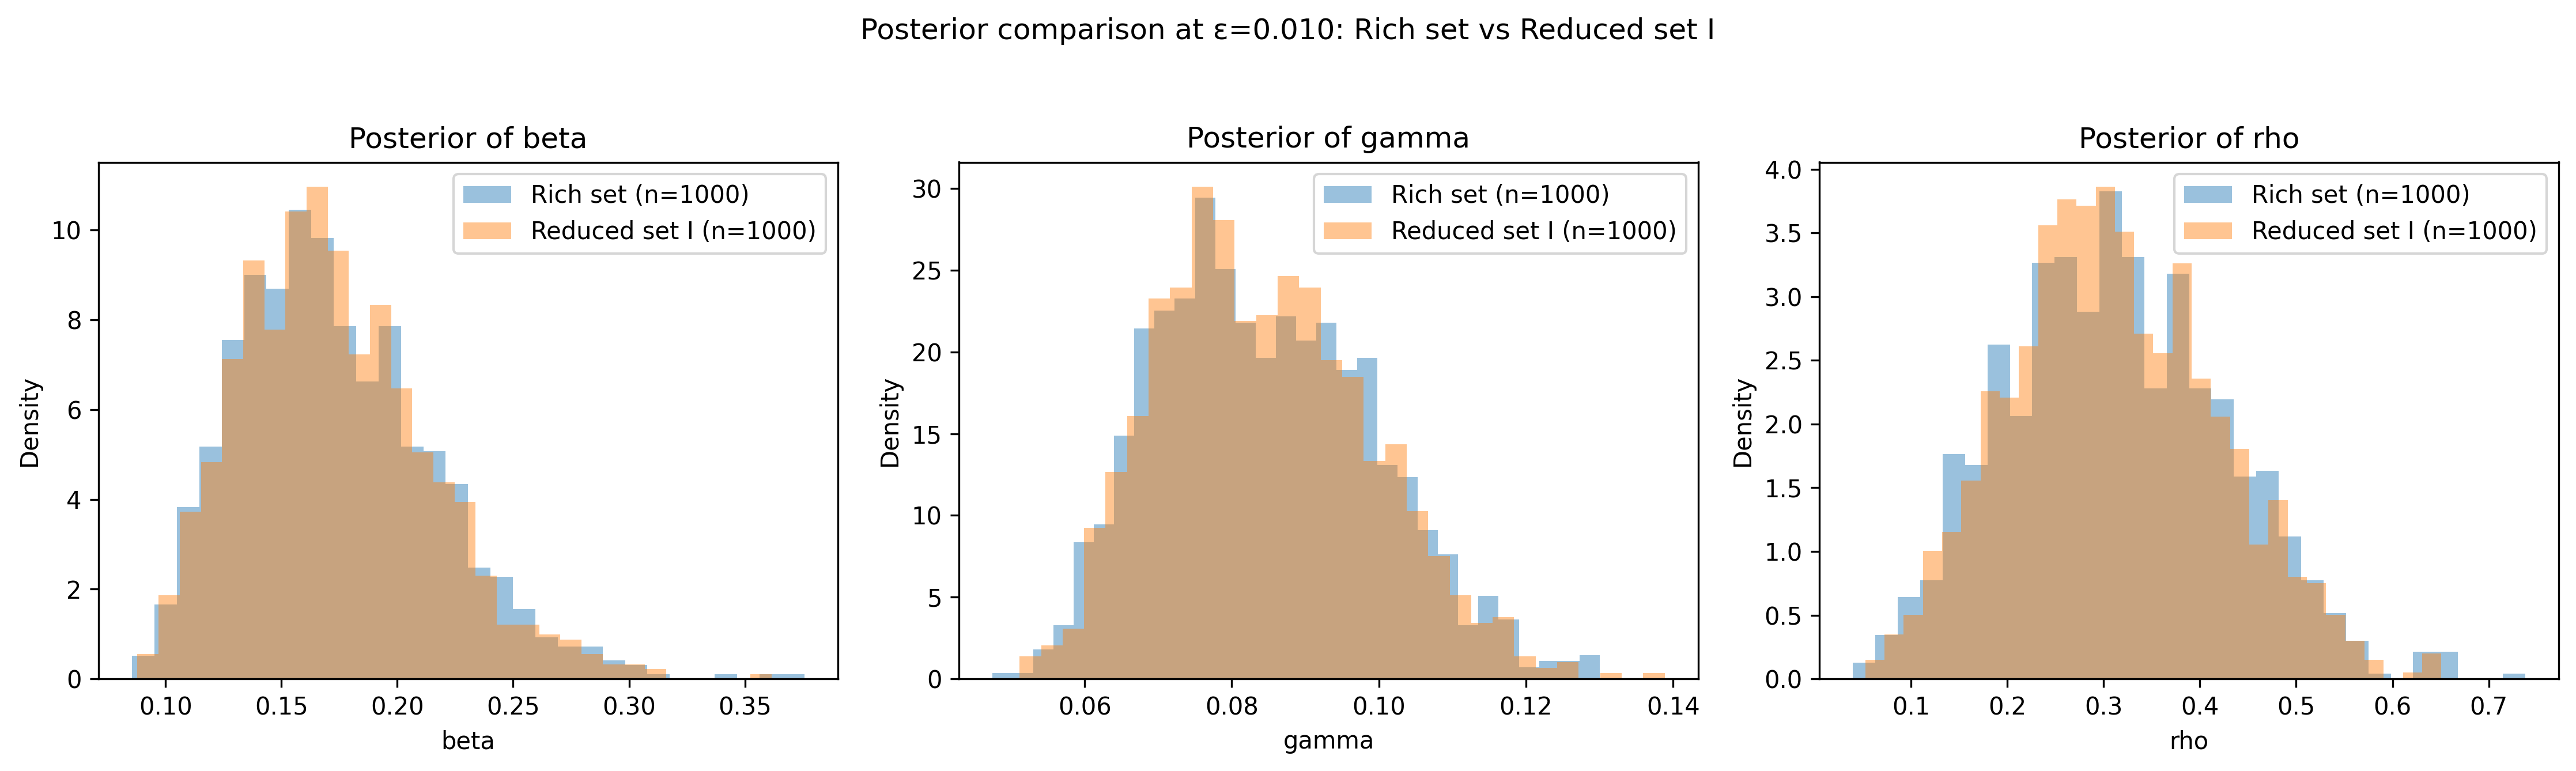
\includegraphics[width=\linewidth]{outputs/basic_abc/summary_set_study/posterior_rich_set_vs_reduced_set_i_eps-0.0100_2026-04-12_23-11.png}
    \caption{Rich set versus Reduced set I.}
\end{subfigure}
\hfill
\begin{subfigure}[t]{0.48\textwidth}
    \centering
    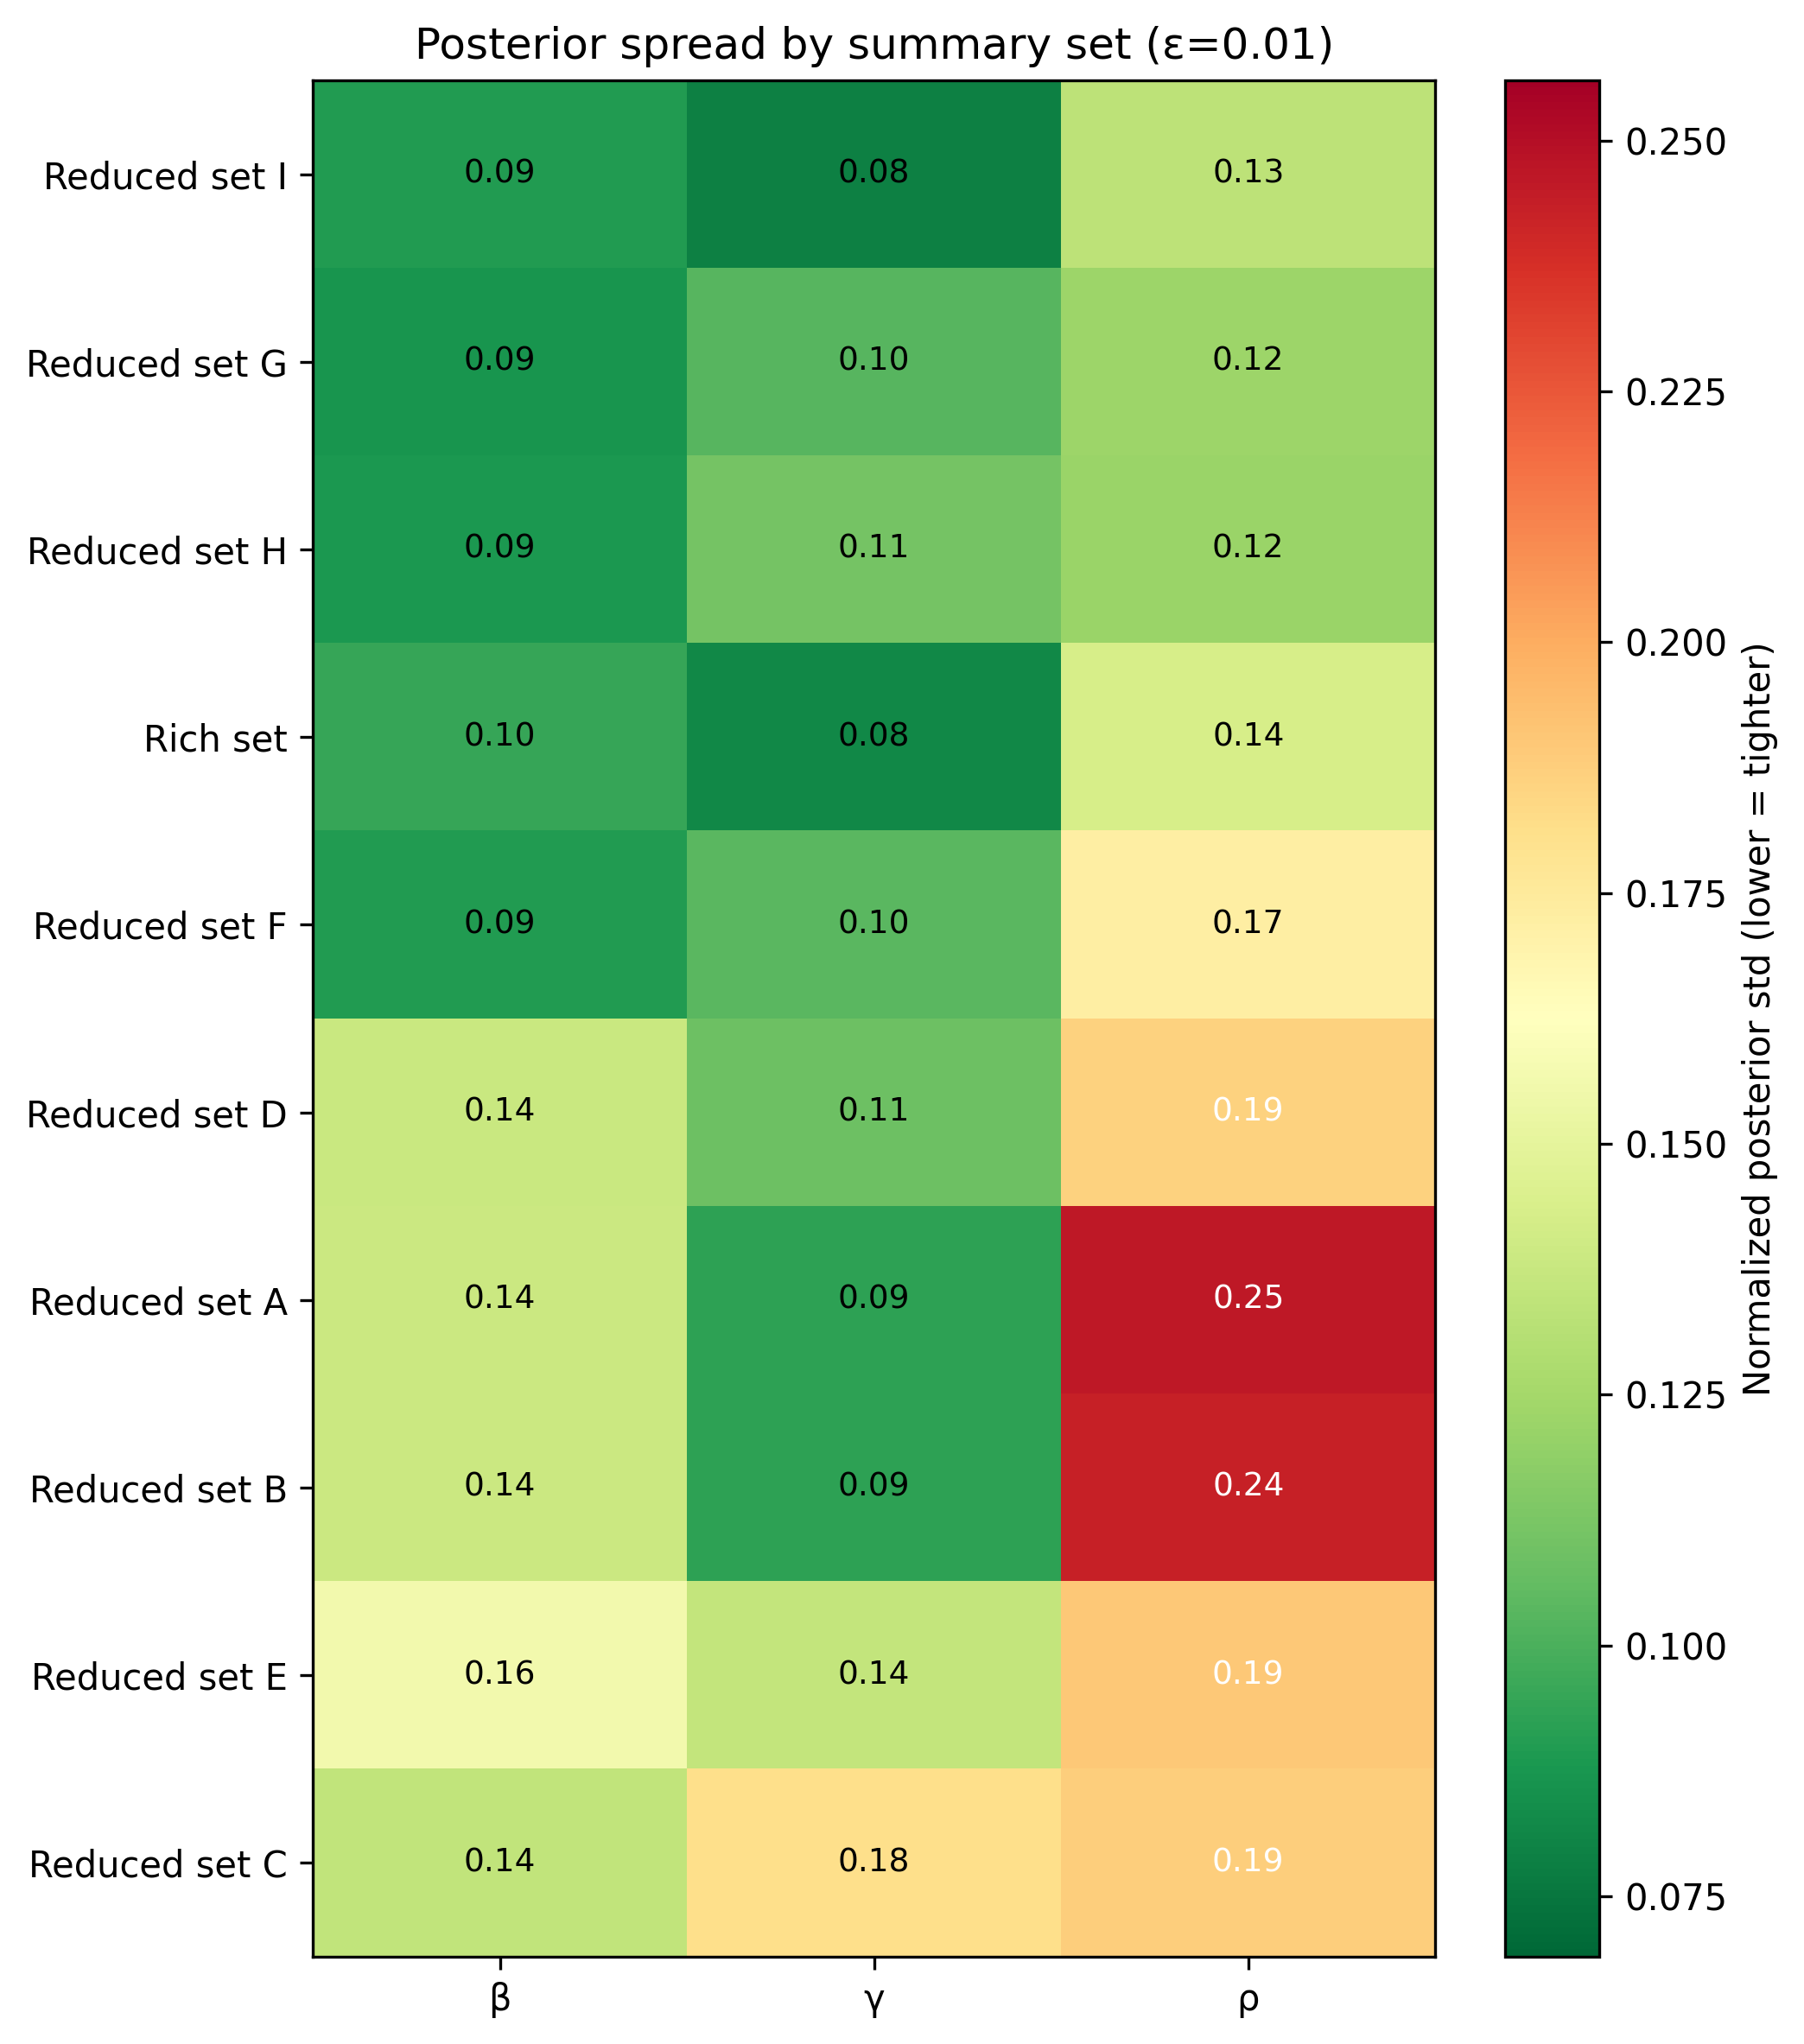
\includegraphics[width=\linewidth]{outputs/basic_abc/summary_set_study/posterior_spread_heatmap_2026-04-12_23-12.png}
    \caption{Posterior-spread heatmap.}
\end{subfigure}
\caption{Critical summary-set selection evidence from \texttt{abc\_rejection.py}. Reduced set I preserves the rich-set posterior while also achieving the smallest mean normalized posterior spread.}
\label{fig:summary-set-selection}
\end{figure}

The heatmap adds a second criterion: posterior concentration. Its normalized posterior-spread scores give Reduced set I the smallest mean spread among the tested summary sets, approximately $0.101$, compared with $0.107$ for the rich set itself. The interpretation is not simply that tighter is better. Rather, Reduced set I is attractive because it stays visually faithful to the rich-set benchmark while slightly reducing posterior dispersion, suggesting that the omitted rich-set summaries were mostly redundant or noisy for this problem.

For the rest of the report, Reduced set I is therefore used as the reduced-summary reference posterior. This is also the subset exported by \texttt{abc\_rejection.py} into \texttt{data/intermediate/abc\_rejection\_output.npz} for downstream algorithms. All later extensions inherit that choice directly, so the regression-adjustment, ABC-MCMC, and SMC-ABC analyses are all conditioned on the same Reduced set I calibration.

\section{Extensions Beyond ABC-Rejection Posteriors}

The methods in this section are motivated by the SBI literature on improving efficiency or reducing approximation bias beyond basic rejection ABC. In particular, regression adjustment follows the local-linear correction idea of \citet{beaumont2002}, ABC-MCMC follows the likelihood-free MCMC construction of \citet{marjoram2003}, and SMC-ABC uses a sequential population update with progressively smaller distance thresholds.

\subsection{Regression Adjusted}

The script \texttt{abc\_rejection\_regression.py} now reads the Reduced set I calibration exported by \texttt{abc\_rejection.py} from \texttt{data/intermediate/abc\_rejection\_output.npz}. The regression adjustment therefore operates on the same standardized six-dimensional summary vector used by the updated rejection reference posterior,
\[
(s_1,s_2,s_4,s_5,s_7,s_8),
\]
that is, maximum infection fraction, time to peak, early rewiring growth, degree variance, rewiring per infection, and infection peak width at half maximum. If $\theta_i$ is an accepted parameter draw and $s_i$ is its accepted summary vector, the adjustment is of the form
\[
\theta_i^{\text{adj}} = \theta_i - (s_i - s_{\text{obs}})^\top \widehat{b},
\]
where $\widehat{b}$ is estimated by weighted linear regression of parameters on accepted summaries. The weights are Epanechnikov-style kernel weights based on the accepted distances:
\[
w_i = 1 - \left(\frac{d_i}{h}\right)^2,
\]
with $h$ equal to the largest accepted distance in the reference rejection sample. Intuitively, this tries to remove the local linear bias that remains because the accepted summaries are close to, but not exactly equal to, the observed summaries.

In the current script, the same saved rejection reference pool is also reused to construct looser accepted sets at $\epsilon \in \{0.05,0.10\}$ without rerunning the simulator. This makes it possible to study whether local-linear adjustment allows a less restrictive acceptance threshold while preserving essentially the same posterior.

In implementation terms, \texttt{abc\_rejection\_regression.py} reuses the saved rejection-reference pool, forms accepted subsets at $\epsilon \in \{0.01,0.05,0.10\}$ by thresholding the saved distances, applies Epanechnikov weights inside each accepted subset, and fits a separate weighted linear regression for each of $\beta$, $\gamma$, and $\rho$ on the accepted summary vectors. Those fitted local slopes are then used to adjust each accepted draw back toward the observed summary vector before the script saves the adjusted posterior samples and the cross-$\epsilon$ overlay plots.

Figure~\ref{fig:regression-adjustment} highlights the two most informative new regression plots. The left subfigure is the projected-summary-discrepancy diagnostic at $\epsilon=0.01$. There is a clear positive linear trend in all three parameter panels, especially for $\rho$: when the projected discrepancy is positive, the accepted parameter values tend to be larger, and when it is negative, they tend to be smaller. Accepted samples to the right of zero tend to overshoot the adjusted posterior mean, while those to the left tend to undershoot it, so a local linear correction is exactly the appropriate response. The right panel overlays the regression-adjusted posteriors at $\epsilon=0.01$, $\epsilon=0.05$, and $\epsilon=0.10$.

\begin{figure}[H]
\centering
\begin{subfigure}[t]{0.48\textwidth}
    \centering
    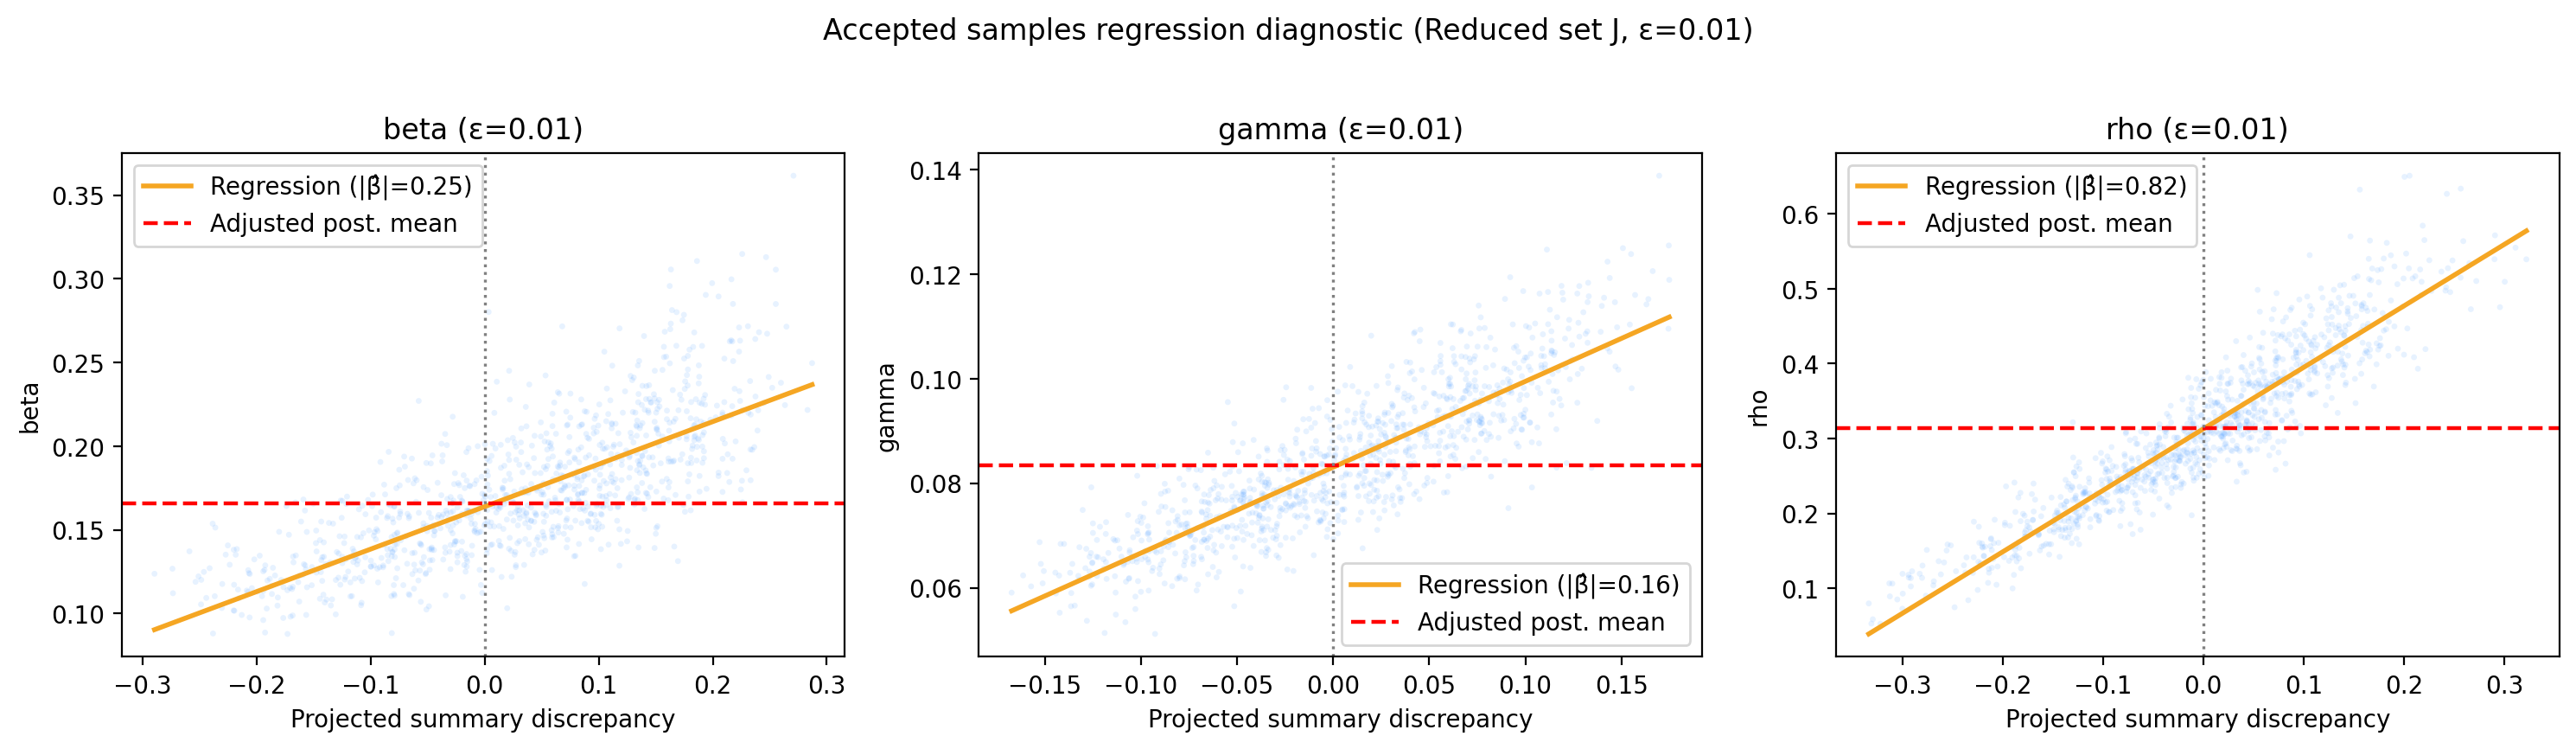
\includegraphics[width=\linewidth]{outputs/regression_adjustment/plots/regression_projection_diagnostic_eps-0.0100.png}
    \caption{Projected-discrepancy diagnostic at $\epsilon=0.01$.}
\end{subfigure}
\hfill
\begin{subfigure}[t]{0.48\textwidth}
    \centering
    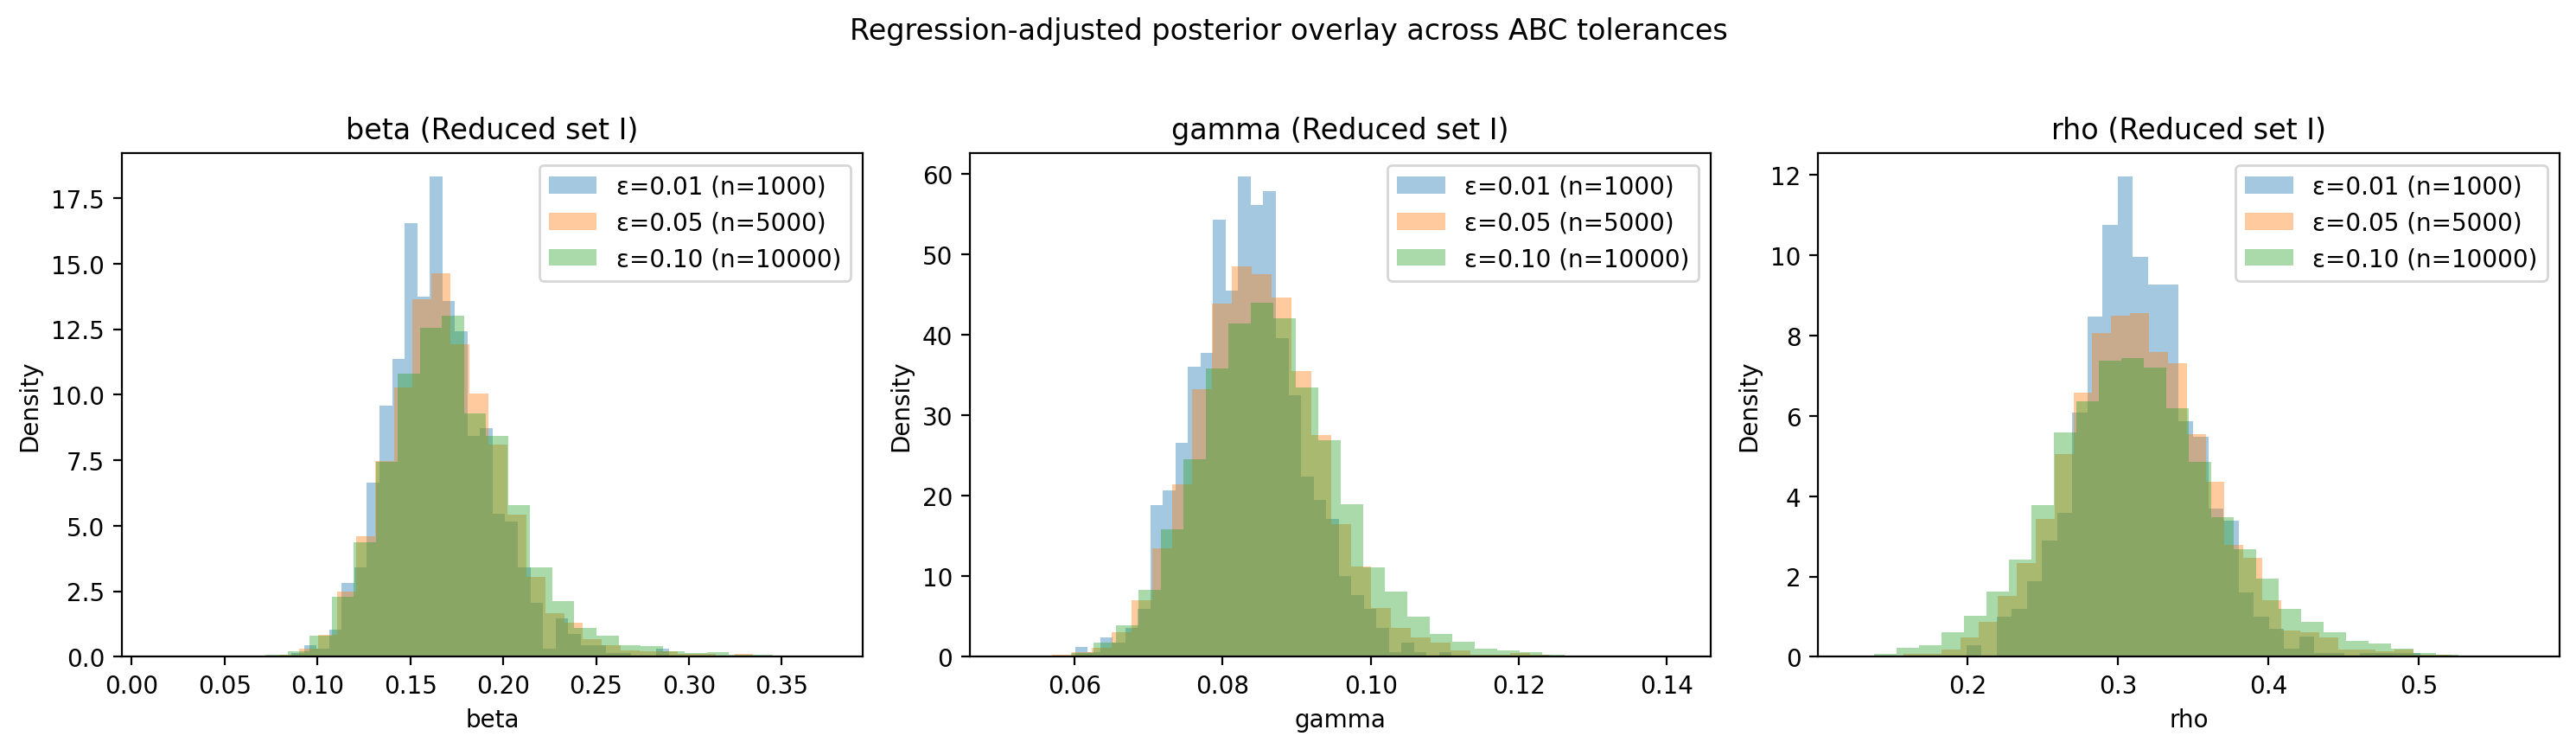
\includegraphics[width=\linewidth]{outputs/regression_adjustment/plots/posterior_overlay_regression_adjustment_across_epsilons.png}
    \caption{Adjusted posterior overlay across tolerances.}
\end{subfigure}
\caption{Key regression-adjustment diagnostics generated by \texttt{abc\_rejection\_regression.py}.}
\label{fig:regression-adjustment}
\end{figure}

Numerically, the adjusted posterior means are
\[
\epsilon=0.01: (0.1656,\ 0.0833,\ 0.3145), \qquad
\epsilon=0.05: (0.1708,\ 0.0851,\ 0.3144), \qquad
\epsilon=0.10: (0.1734,\ 0.0866,\ 0.3130).
\]
The key comparison is between $\epsilon=0.01$ and $\epsilon=0.05$. Their adjusted posterior centers are extremely close, and the corresponding 95\% interval for $\rho$ changes only from $[0.2390,\ 0.3945]$ to $[0.2233,\ 0.4191]$. By contrast, $\epsilon=0.10$ begins to show more visible tail inflation, especially for $\rho$. This is a useful statistical point: once regression adjustment is applied, the strictest tolerance is not automatically optimal. A looser tolerance such as $\epsilon=0.05$ uses many more accepted draws from the same reference pool ($5000$ rather than $1000$), so the fitted regression coefficients have lower Monte Carlo variance while the adjusted posterior remains nearly unchanged. In that sense, a moderately looser tolerance can actually give a higher-quality regression-adjusted posterior: it is smoother and more stable because the local linear correction is estimated from a larger accepted sample, yet it does not introduce any material shift in the posterior center.

\subsection{ABC-MCMC}

The next extension is implemented in \texttt{abc\_mcmc.py}. It follows the basic idea of performing MCMC while replacing the unavailable likelihood evaluation with an ABC acceptance rule \citep{marjoram2003}. Rather than recalibrating the problem from scratch, the script loads the updated Reduced set I rejection output from \texttt{data/intermediate/abc\_rejection\_output.npz}. This ensures that the summary subset, standardization constants, observed summary vector, and distance threshold are exactly the same as in the reference rejection run, making the comparison fair after the upstream changes to \texttt{abc\_rejection.py}.

The proposal mechanism is a Gaussian random walk with componentwise scales
\[
(0.035,\ 0.012,\ 0.06)
\]
for $(\beta,\gamma,\rho)$ respectively, constrained to remain within the original uniform prior support. The script runs $30{,}000$ proposals, stores $30{,}001$ chain states including the initial accepted state, discards the first $3{,}000$ iterations as burn-in, and retains $27{,}001$ posterior samples. The fixed ABC distance threshold loaded from the rejection calibration is
\[
\tau = 0.545343.
\]

In the actual implementation, \texttt{abc\_mcmc.py} starts from an accepted rejection draw, proposes Gaussian random-walk moves inside the original prior box, simulates the full eight-summary vector for each proposal, retains only the Reduced set I components $(s_1,s_2,s_4,s_5,s_7,s_8)$, and accepts the proposal whenever its standardized ABC distance is finite and does not exceed the saved rejection threshold $\tau$. Because the proposal is symmetric and the prior is uniform on a rectangular support, this fixed-threshold ABC rule is the entire accept/reject mechanism.

The saved diagnostics in \texttt{outputs/abc\_mcmc/abc\_mcmc\_diagnostics.csv} report an acceptance rate of $0.1894$. Figure~\ref{fig:mcmc-trace} shows the trace plots, and Figure~\ref{fig:mcmc-comparison} compares the MCMC posterior against the Reduced set I rejection posterior used as its reference.

\begin{figure}[H]
\centering
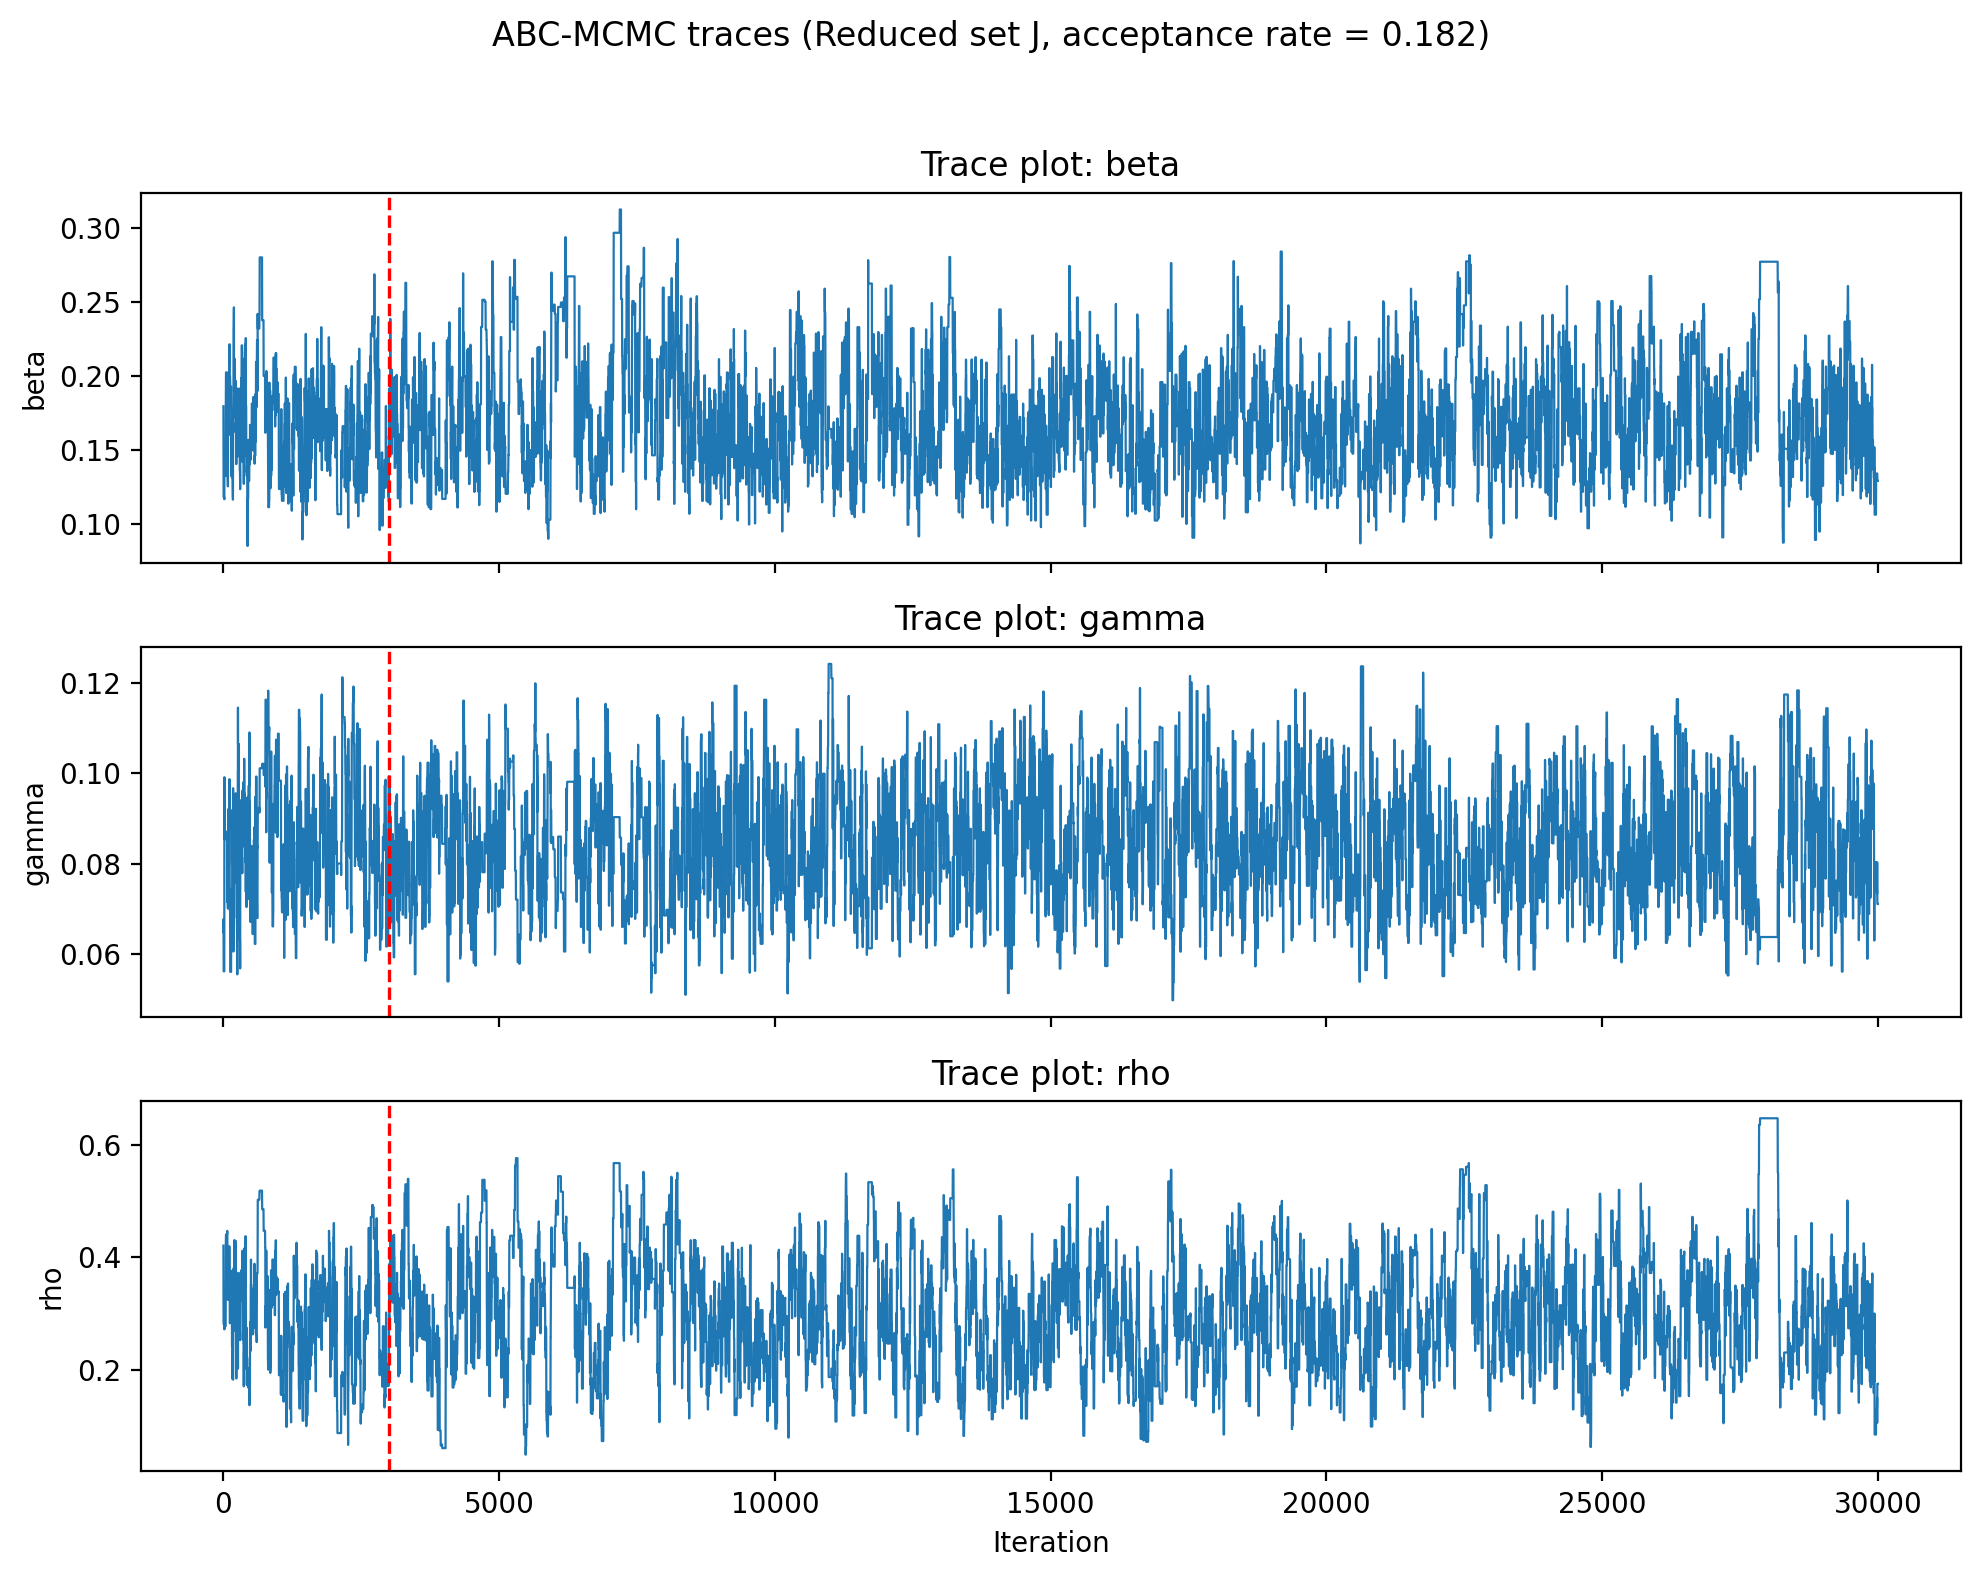
\includegraphics[width=0.76\textwidth]{outputs/abc_mcmc/plots/abc_mcmc_trace_plots.png}
\caption{ABC-MCMC trace plots generated by \texttt{abc\_mcmc.py}. The dashed line marks the burn-in cutoff at iteration $3000$.}
\label{fig:mcmc-trace}
\end{figure}

\begin{figure}[H]
\centering
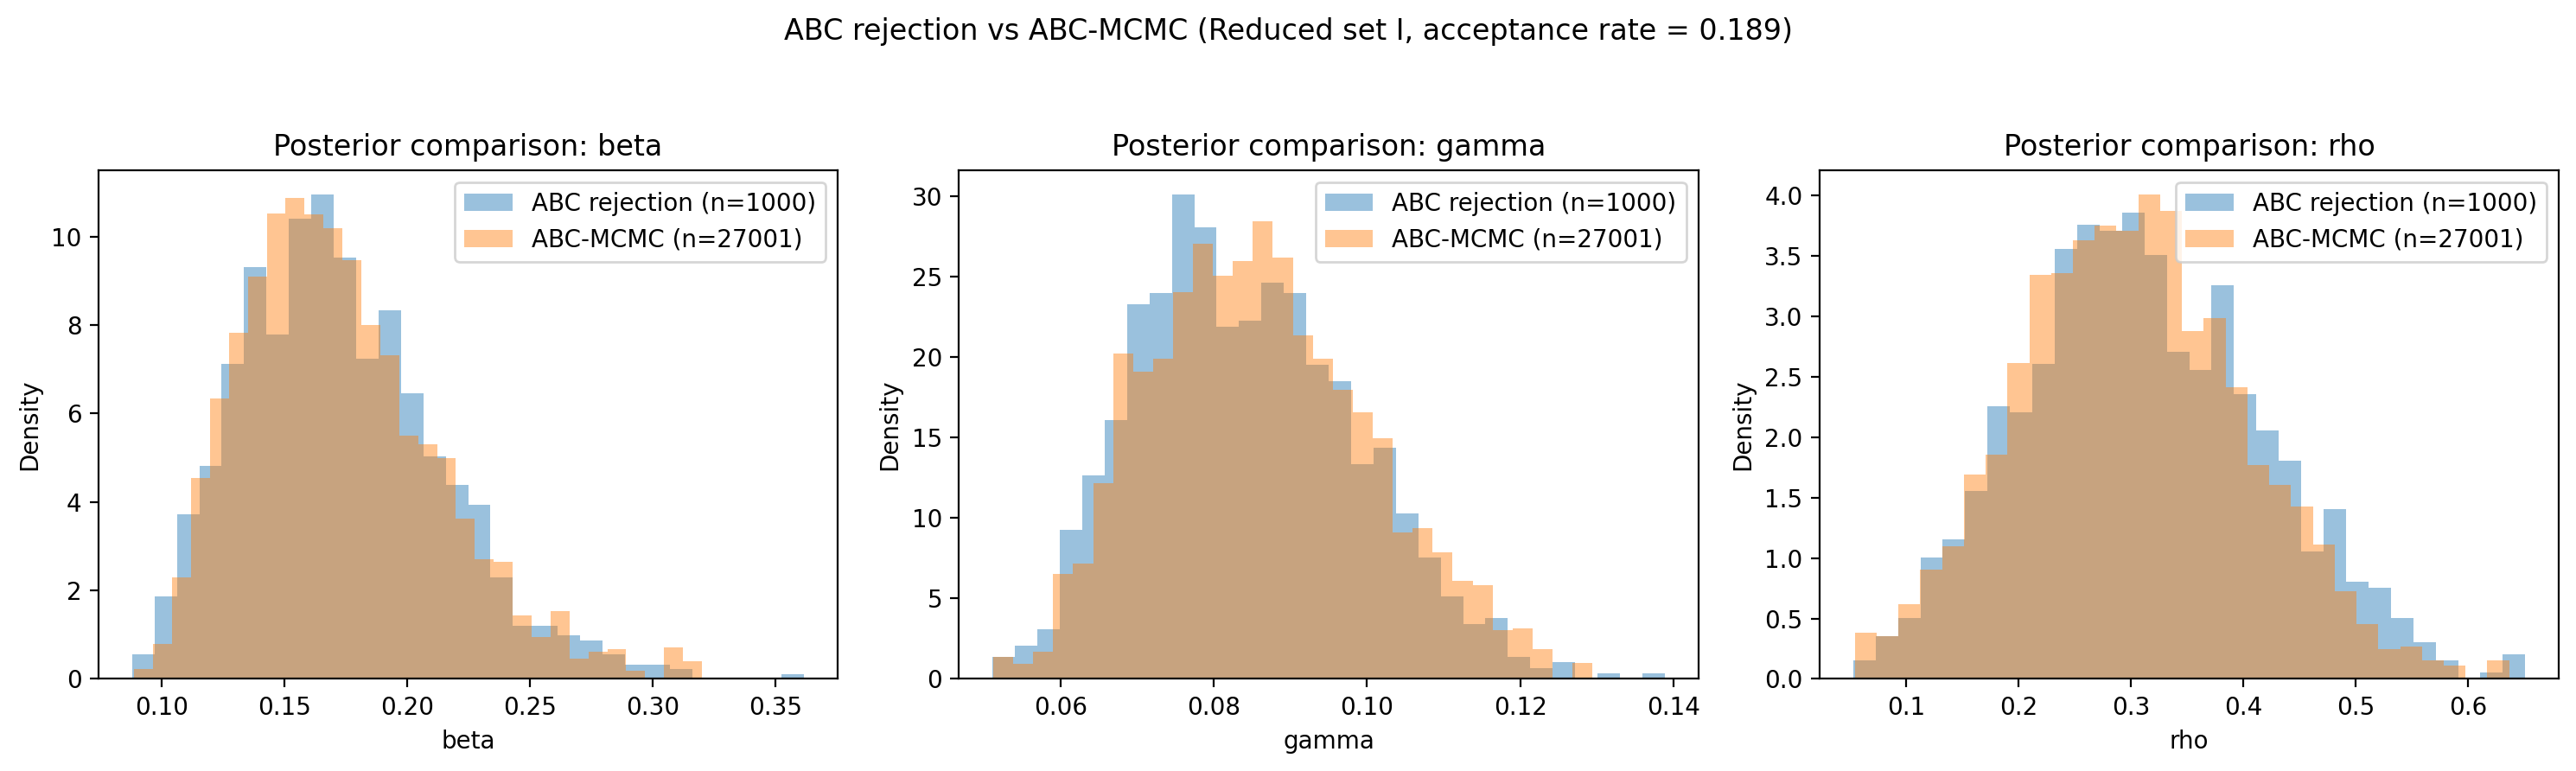
\includegraphics[width=0.76\textwidth]{outputs/abc_mcmc/plots/abc_rejection_vs_mcmc_posterior_histograms.png}
\caption{Posterior comparison between Reduced set I rejection ABC and ABC-MCMC.}
\label{fig:mcmc-comparison}
\end{figure}

The MCMC traces do not show obvious divergence or runaway behavior. They exhibit persistent local dependence, which is expected for a random-walk chain, but they still explore the same high-density regions found by rejection ABC. This is consistent with the workable acceptance rate of about $18.9\%$.

The posterior means from the retained ABC-MCMC sample are
\[
(0.1727,\ 0.0861,\ 0.3009),
\]
with empirical 95\% posterior intervals
\[
\beta \in [0.1114,\ 0.2635], \qquad
\gamma \in [0.0614,\ 0.1163], \qquad
\rho \in [0.1100,\ 0.5086].
\]
These are extremely close to the Reduced set I rejection posterior
\[
(0.1730,\ 0.0844,\ 0.3109),
\]
which suggests that the basic rejection sample already captures the main posterior mass well. The practical advantage of ABC-MCMC is therefore not that it radically changes the answer, but that it provides a much larger posterior sample under the same ABC target while preserving the same inferential conclusions.

\subsection{SMC-ABC}

The script \texttt{smc\_abc.py} implements a sequential Monte Carlo ABC extension on the same Reduced set I summary statistics exported by \texttt{abc\_rejection.py}. Unlike ABC-MCMC, which keeps a fixed distance threshold throughout the run, SMC-ABC evolves a particle population across a sequence of increasingly strict distance thresholds. In the current run, the four stages target the cumulative quantile thresholds
\[
(0.10,\ 0.05,\ 0.02,\ 0.01),
\]
which correspond to the realized distance thresholds
\[
(1.0221,\ 0.8202,\ 0.6384,\ 0.5430),
\]
with $N=300$ particles at each stage. The first stage samples from the prior until the simulated summary vector falls within the stage-1 distance threshold, while later stages resample particles according to their current weights, perturb them with a Gaussian kernel, and retain only proposals that satisfy the tighter threshold. In implementation terms, the adaptive updates use the relative quantile reductions
\[
0.05/0.10 = 0.50, \qquad 0.02/0.05 = 0.40, \qquad 0.01/0.02 = 0.50,
\]
applied to the accepted distance distribution of the previous SMC population.

The saved diagnostics in \texttt{outputs/smc\_abc/smc\_abc\_diagnostics.csv} show the expected efficiency pattern as the target region contracts. The stagewise acceptance rates decrease from $10.94\%$ to $10.62\%$, $9.81\%$, and finally $8.59\%$. At the same time, the effective sample size remains high, moving only from $300.0$ in stage 1 to $289.6$, $280.3$, and $268.4$ by stage 4. This indicates that the particle system does not collapse severely even though the distance threshold becomes substantially tighter. The final adaptive threshold, $0.5430$, is also very close to the rejection reference threshold $0.5453$, so the final SMC target remains directly comparable with the updated basic-ABC baseline.

Figure~\ref{fig:smc-results} summarizes the SMC-ABC results. The left column compares the final SMC-ABC posterior against the Reduced set I rejection posterior used as reference, while the right column shows the stage-by-stage evolution of the SMC particle populations. The comparison histograms use matched sample counts, so visible differences are not artifacts of one method contributing many more draws than the other. The overlap is strong for all three parameters. The SMC-ABC posterior means are
\[
(0.1747,\ 0.0836,\ 0.3094),
\]
which are close to the corresponding rejection-ABC means
\[
(0.1730,\ 0.0844,\ 0.3109).
\]
For $\beta$ and $\gamma$, the SMC and rejection posteriors are nearly indistinguishable in location, differing mainly through a mild smoothing of the histogram shape. For $\rho$, the SMC posterior is still centered in the same broad region but exhibits a slightly heavier upper tail. The 95\% posterior intervals from SMC-ABC are
\[
\beta \in [0.1083,\ 0.2847], \qquad
\gamma \in [0.0608,\ 0.1122], \qquad
\rho \in [0.1278,\ 0.5144].
\]
Compared with the rejection reference, the intervals for $\beta$ and especially $\rho$ are somewhat wider, but the substantive interpretation remains unchanged.

The right-column progression plots in Figure~\ref{fig:smc-results} show how the SMC populations evolve across stages. The posterior for $\beta$ tightens most visibly, with the highest-density region settling around roughly $0.14$ to $0.20$ by the final stage and the large-$\beta$ tail shrinking relative to stage 1. The posterior for $\gamma$ also becomes more concentrated, but the effect is more modest, and stages 3 and 4 already look very similar. By contrast, the posterior for $\rho$ remains diffuse across all four stages. Although the later stages reduce some mass in the extreme upper tail, the distribution of $\rho$ is still broad at the final threshold. This suggests that, under the chosen summary statistics, $\beta$ and $\gamma$ are identified more sharply than $\rho$.

Taken together, the SMC results reinforce the same inferential conclusions seen earlier from rejection ABC and ABC-MCMC. Sequential tightening of the distance threshold does not materially shift the posterior center, but it confirms that the posterior structure is stable under a different sampling mechanism. The main practical gain from SMC-ABC in this setting is therefore efficiency in reaching smaller distance thresholds while preserving the same qualitative conclusions: $\beta$ and $\gamma$ are moderately well pinned down, whereas $\rho$ remains the least precisely identified parameter.

\subsubsection{Synthetic Truth Recovery}

To validate the reliability of the SMC-ABC pipeline, we performed a synthetic-truth recovery run implemented in \texttt{synthetic\_recovery\_smc\_abc.py}. In this experiment, the "observed" data is replaced by a single synthetic realization generated from known ground-truth parameters:
\[
\theta^* = (\beta^*, \gamma^*, \rho^*) = (0.25, 0.08, 0.40).
\]
This allows us to evaluate whether the posterior distribution correctly covers the true parameter values under the same summary-statistic configuration (Reduced set I) used throughout the report.

The methodology follows the standard SMC-ABC workflow, with one additional step: the initial distance threshold is re-calibrated relative to the new synthetic target. Specifically, we recompute the distances of all reference simulations to the synthetic summary vector and set the stage-1 threshold to the $10\%$ quantile of these new distances. The sequential updates then tighten this threshold adaptively across four stages.

The recovery diagnostics in \texttt{outputs/smc\_abc\_recovery/recovery\_diagnostics.csv} show that the algorithm converged through the adaptive distance schedule
\[
(0.9664,\ 0.7451,\ 0.5550,\ 0.4670),
\]
maintaining a robust effective sample size ($ESS \approx 277$) and a workable final acceptance rate of $6.08\%$.

Figure~\ref{fig:recovery-results} presents the recovery posteriors. In all three panels, the true parameter value (marked by the \textcolor{red}{red dashed line}) lies well within the high-density region of the SMC-ABC posterior.
For $\beta$ and $\gamma$, the posterior is relatively concentrated around the truth, with means of $0.2183$ and $0.0818$ respectively. For $\rho$, while the posterior is broader, the true value of $0.40$ is clearly captured within the main mass of the distribution (posterior mean $0.3582$).

\begin{figure}[H]
\centering
\begin{subfigure}[t]{0.32\textwidth}
    \centering
    \includegraphics[width=\linewidth]{outputs/smc_abc_recovery/plots/recovery_beta.png}
    \caption{$\beta$ recovery.}
\end{subfigure}
\hfill
\begin{subfigure}[t]{0.32\textwidth}
    \centering
    \includegraphics[width=\linewidth]{outputs/smc_abc_recovery/plots/recovery_gamma.png}
    \caption{$\gamma$ recovery.}
\end{subfigure}
\hfill
\begin{subfigure}[t]{0.32\textwidth}
    \centering
    \includegraphics[width=\linewidth]{outputs/smc_abc_recovery/plots/recovery_rho.png}
    \caption{$\rho$ recovery.}
\end{subfigure}
\caption{Synthetic truth recovery results. The \textcolor{red}{red dashed lines} indicate the true parameter values $(\beta^*=0.25, \gamma^*=0.08, \rho^*=0.40)$ used to generate the synthetic observed data.}
\label{fig:recovery-results}
\end{figure}

The success of this recovery run provides empirical evidence that the current Reduced set I summary statistics are informative for the model parameters and that the SMC-ABC pipeline is capable of producing a posterior that is consistent with the ground truth. This increases our confidence in the inferences drawn from the actual observed data.

\subsection{Synthetic Likelihood MCMC}

The final extension is the implementation of Synthetic Likelihood MCMC (SL-MCMC), based on the methodology of \citet{wood2010}. Unlike ABC methods that rely on a distance-based kernel, SL-MCMC approximates the likelihood of the summary statistics $s$ using a multivariate Gaussian distribution:
\[
\log L_{SL}(\theta) = -\frac{1}{2} \left[ \log |\Sigma(\theta)| + (s_{\text{obs}} - \mu(\theta))^\top \Sigma(\theta)^{-1} (s_{\text{obs}} - \mu(\theta)) \right]
\]
where $\mu(\theta)$ and $\Sigma(\theta)$ are the mean and covariance matrix of the summaries estimated from simulations at parameter $\theta$. In our implementation, we use $M=30$ simulations per step and apply Ledoit-Wolf shrinkage to regularize the covariance matrix, ensuring numerical stability even when the number of simulations is relatively small. To handle the computational intensity, the pipeline is highly optimized using \texttt{numba} for the SIR simulator and \texttt{multiprocessing} for parallel simulation execution.

\subsubsection{Assumption Check: Normality of Summaries}

The core assumption of SL-MCMC is that the summary statistics follow a multivariate Gaussian distribution. We validated this by simulating $500$ realizations at the posterior mean. Figure~\ref{fig:sl-normality} shows the standardized histograms for the Reduced set I summaries. While some summaries (like Max Infection) exhibit slight skewness, the majority align well with the Normal PDF overlays, and the Shapiro-Wilk p-values suggest that the Gaussian approximation is a reasonable surrogate for the true intractable likelihood in this model.

\begin{figure}[H]
\centering
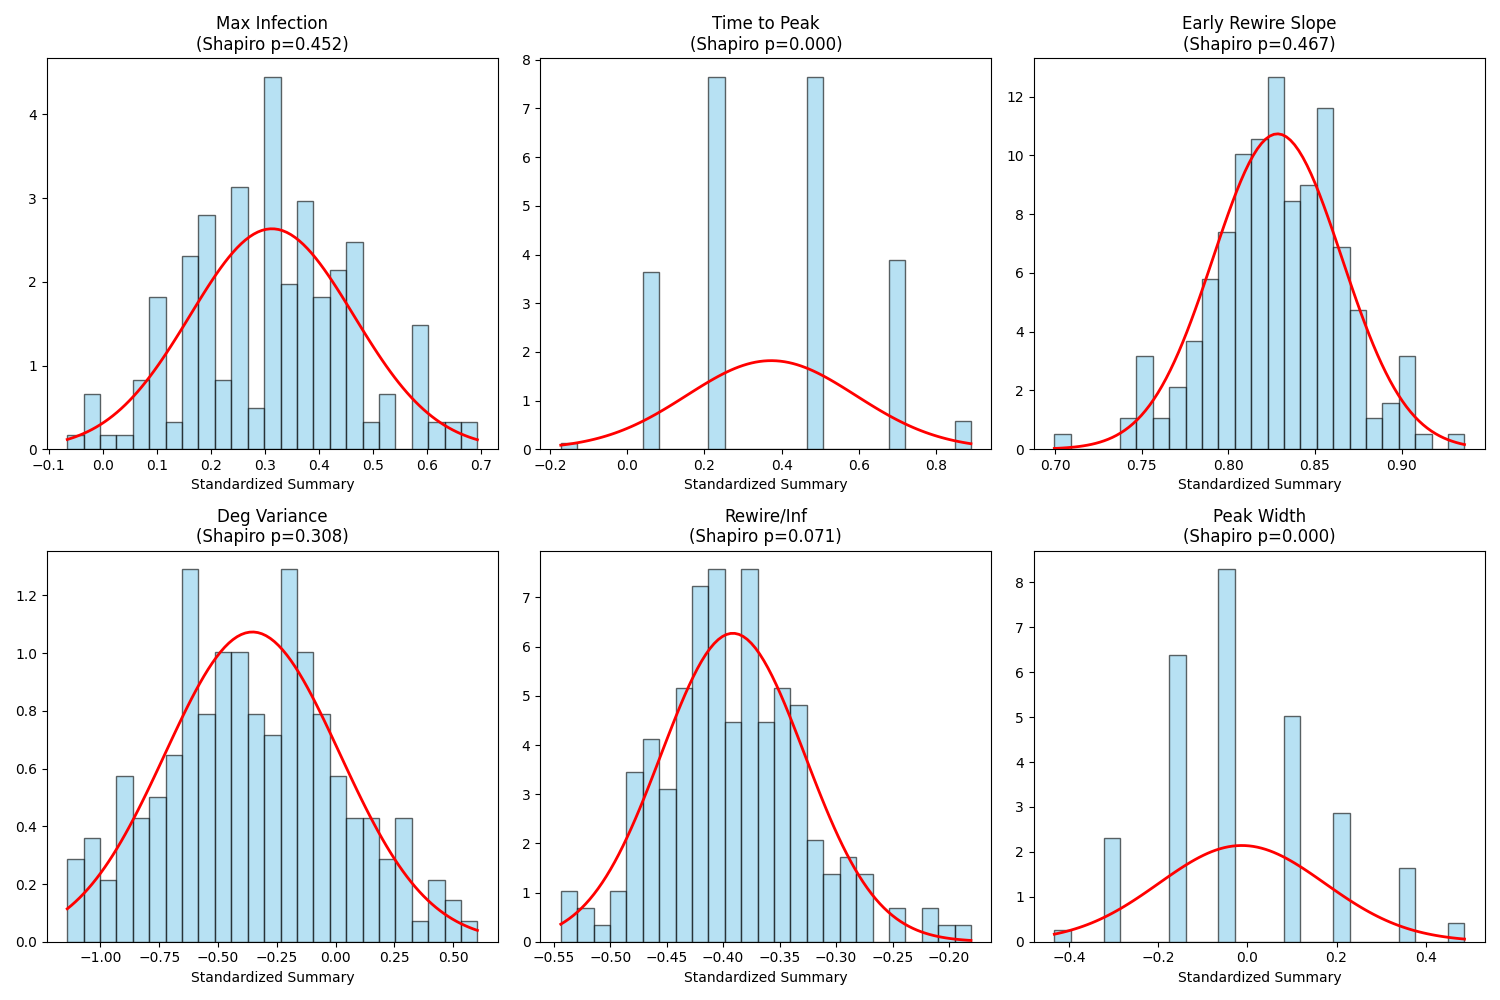
\includegraphics[width=0.85\textwidth]{outputs/synthetic_likelihood_mcmc/diagnostics/assumption_check_normality.png}
\caption{Assumption check for Synthetic Likelihood. Standardized histograms of Reduced set I summaries simulated at the posterior mean show reasonable agreement with the multivariate Gaussian assumption.}
\label{fig:sl-normality}
\end{figure}

\subsubsection{Posterior Comparison and Recovery}

The SL-MCMC was run for $30{,}000$ iterations with a $5{,}000$ iteration burn-in. Figure~\ref{fig:sl-comparison} compares the resulting posterior with the basic ABC rejection ($\epsilon=0.01$) results. The Synthetic Likelihood methodology yields notably sharper and more concentrated posteriors for all three parameters. This increased precision is expected, as SL leverages the full distributional information (mean and covariance) of the summaries rather than collapsing them into a single scalar distance.

\begin{figure}[H]
\centering
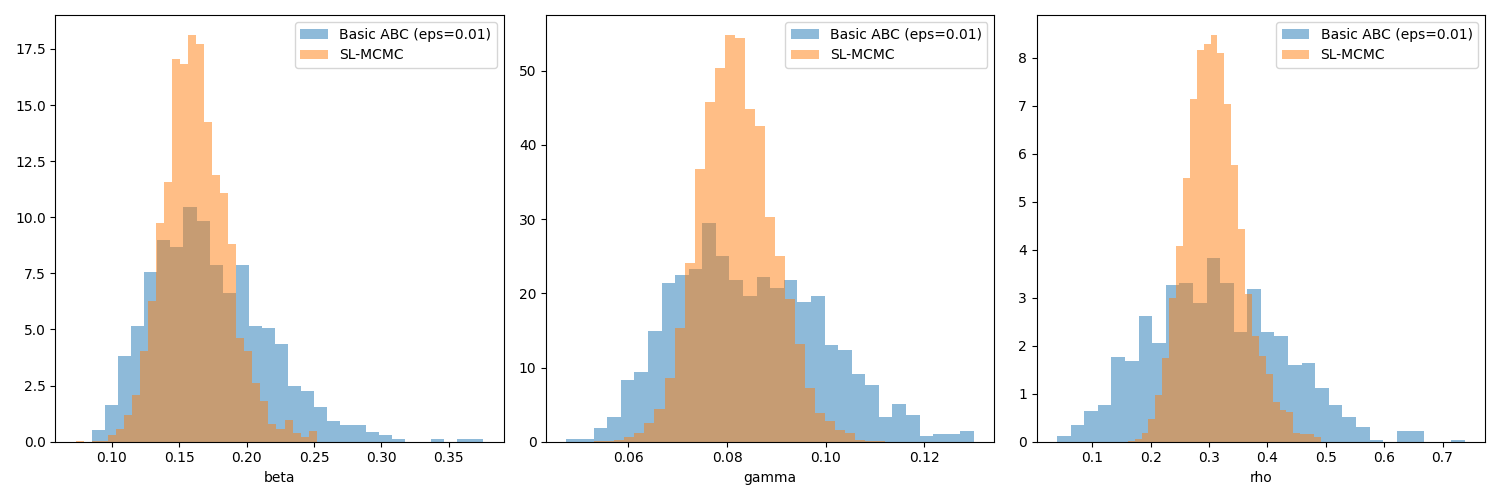
\includegraphics[width=0.85\textwidth]{outputs/synthetic_likelihood_mcmc/plots/synthetic_likelihood_vs_basic_abc_comparison.png}
\caption{Posterior comparison: Basic ABC ($\epsilon=0.01$) versus Synthetic Likelihood MCMC. SL-MCMC provides tighter marginal posteriors, particularly for $\beta$ and $\gamma$.}
\label{fig:sl-comparison}
\end{figure}

Finally, we performed a synthetic-truth recovery run to evaluate the accuracy of the SL pipeline. Using the same ground truth $(\beta^*=0.25, \gamma^*=0.08, \rho^*=0.40)$ as in the SMC-ABC experiment, the SL-MCMC posterior correctly centered around the known values (Figure~\ref{fig:sl-recovery}). The "mean of accepted values" (ground truth) lies squarely within the high-density regions, confirming that the SL-MCMC pipeline can accurately recover the model parameters from known data.

\begin{figure}[H]
\centering
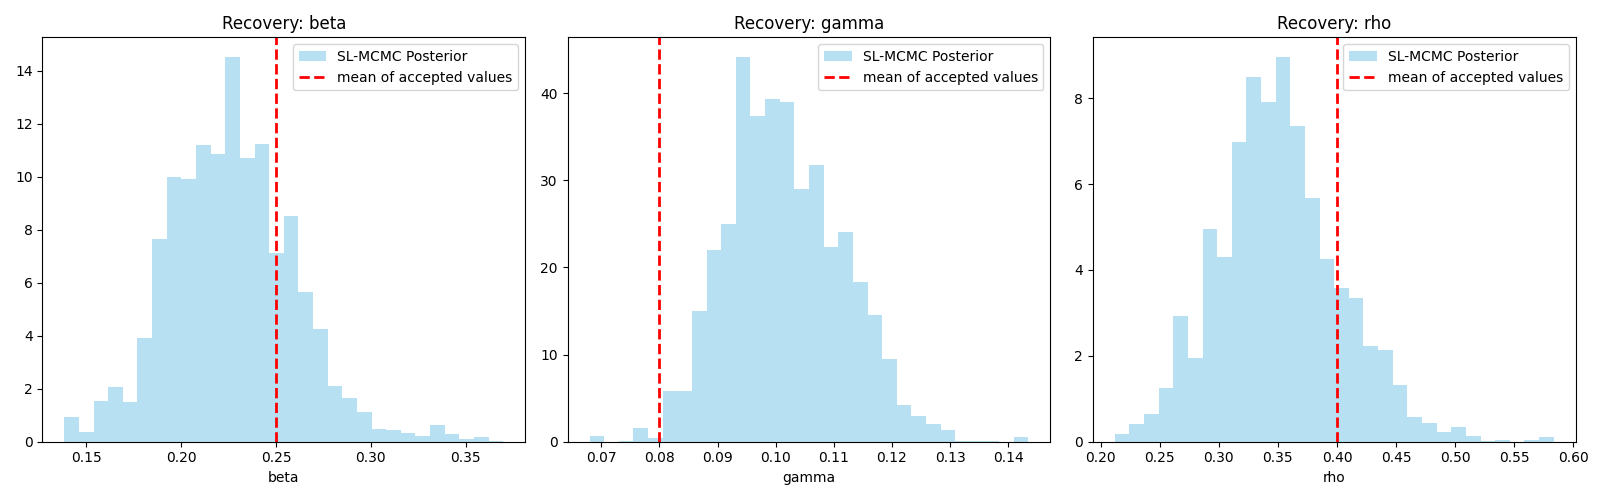
\includegraphics[width=0.85\textwidth]{outputs/sl_mcmc_recovery/plots/synthetic_truth_recovery_sl.png}
\caption{Synthetic truth recovery for SL-MCMC. The \textcolor{red}{red dashed lines} ("mean of accepted values") represent the ground truth parameters used to generate the synthetic target.}
\label{fig:sl-recovery}
\end{figure}

\begin{figure}[H]
\centering
\begin{subfigure}[t]{0.48\textwidth}
    \centering
    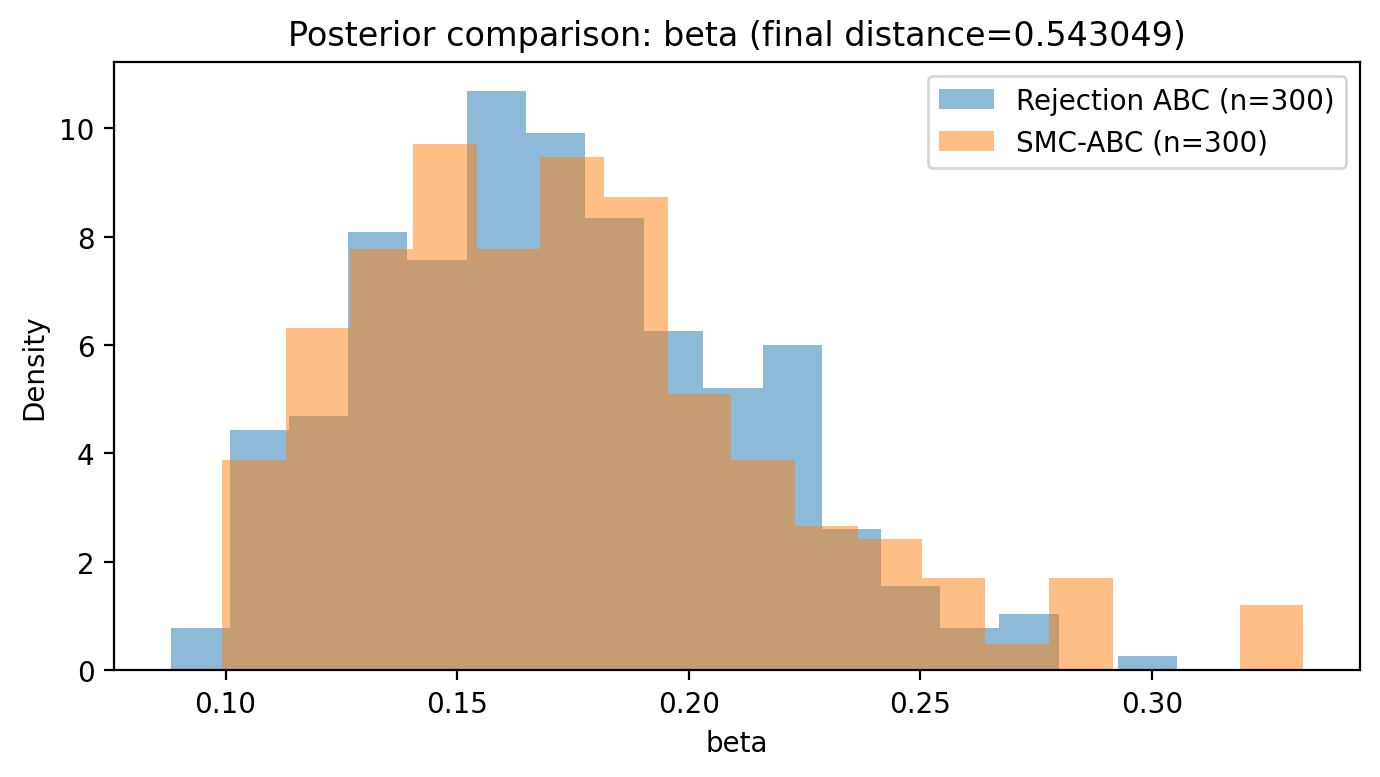
\includegraphics[width=\linewidth]{outputs/smc_abc/plots/beta_rejection_vs_smc_abc.png}
    \caption{$\beta$: rejection ABC versus SMC-ABC.}
\end{subfigure}
\hfill
\begin{subfigure}[t]{0.48\textwidth}
    \centering
    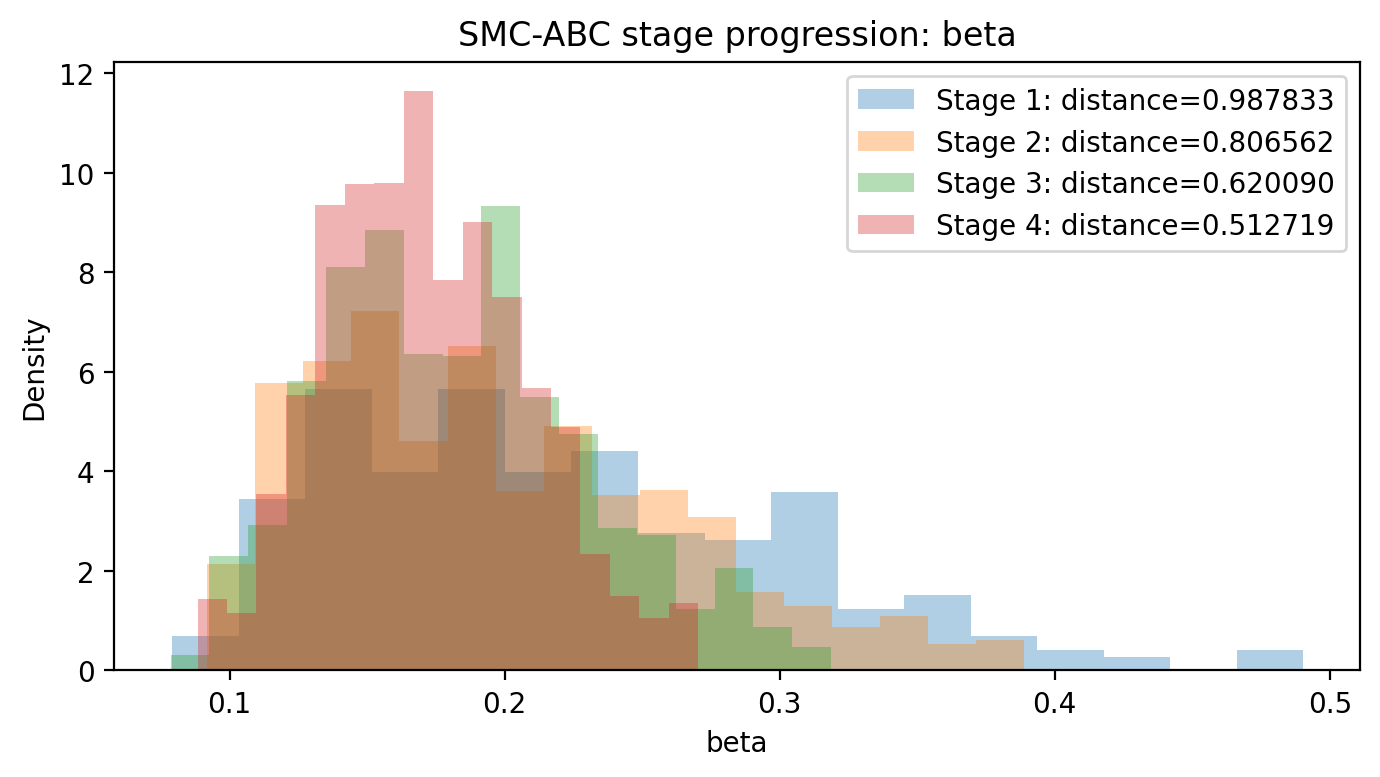
\includegraphics[width=\linewidth]{outputs/smc_abc/plots/beta_smc_abc_stage_progression.png}
    \caption{$\beta$: SMC-ABC stage progression.}
\end{subfigure}

\vspace{0.8em}

\begin{subfigure}[t]{0.48\textwidth}
    \centering
    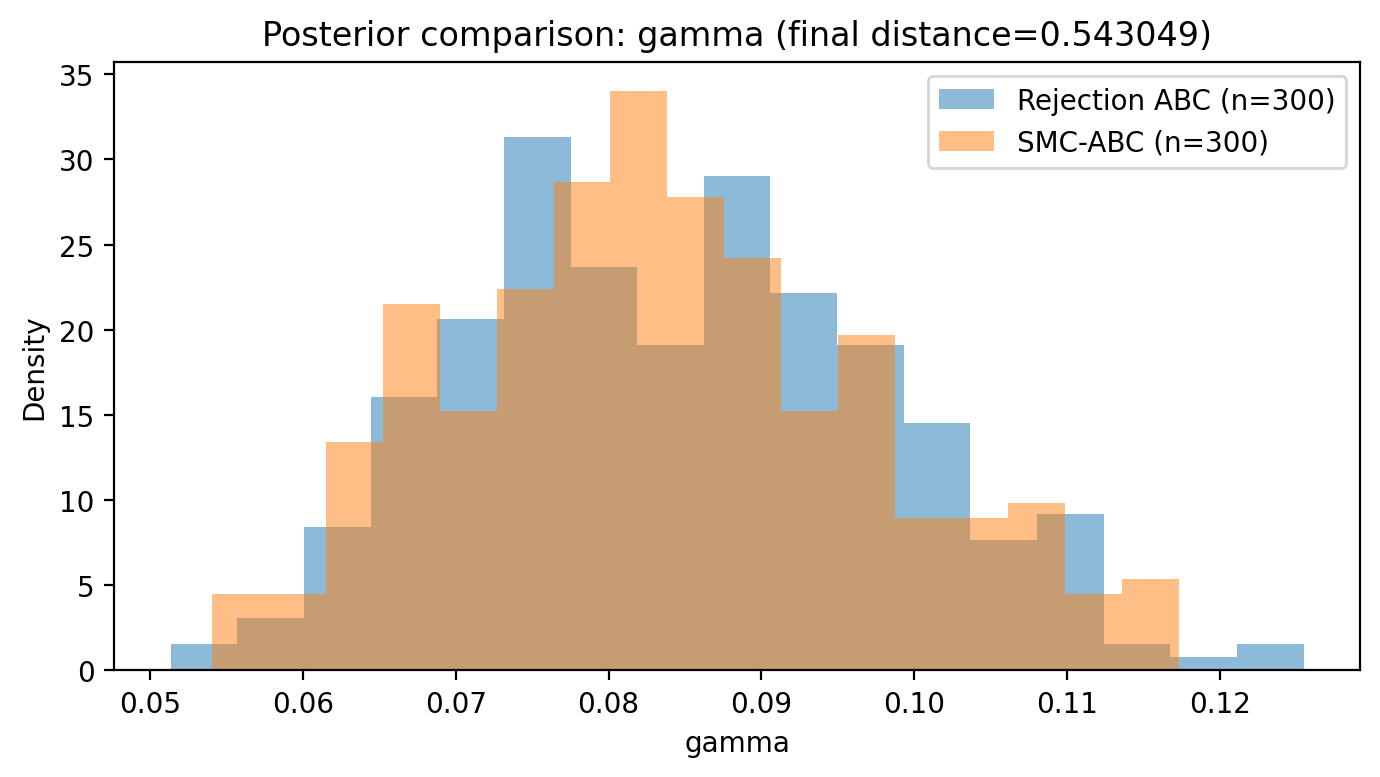
\includegraphics[width=\linewidth]{outputs/smc_abc/plots/gamma_rejection_vs_smc_abc.png}
    \caption{$\gamma$: rejection ABC versus SMC-ABC.}
\end{subfigure}
\hfill
\begin{subfigure}[t]{0.48\textwidth}
    \centering
    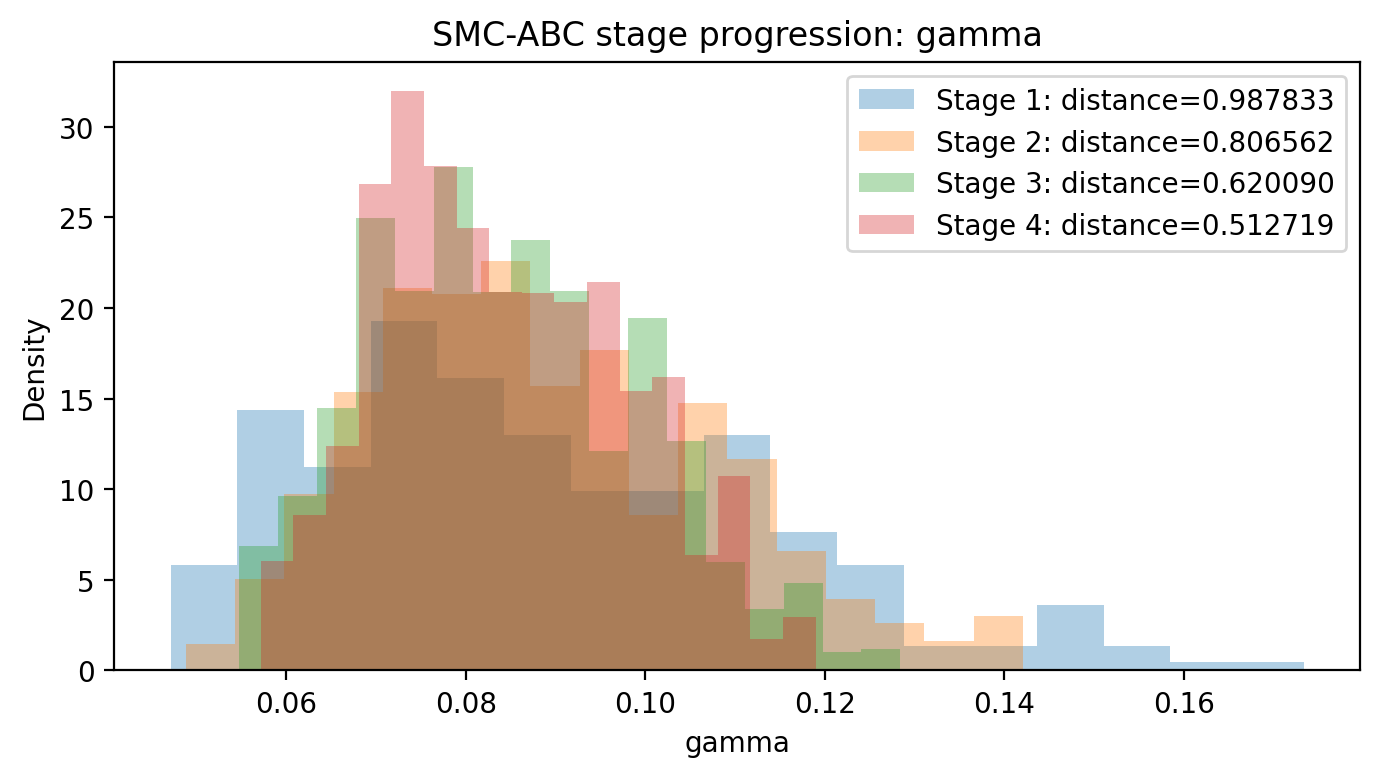
\includegraphics[width=\linewidth]{outputs/smc_abc/plots/gamma_smc_abc_stage_progression.png}
    \caption{$\gamma$: SMC-ABC stage progression.}
\end{subfigure}

\vspace{0.8em}

\begin{subfigure}[t]{0.48\textwidth}
    \centering
    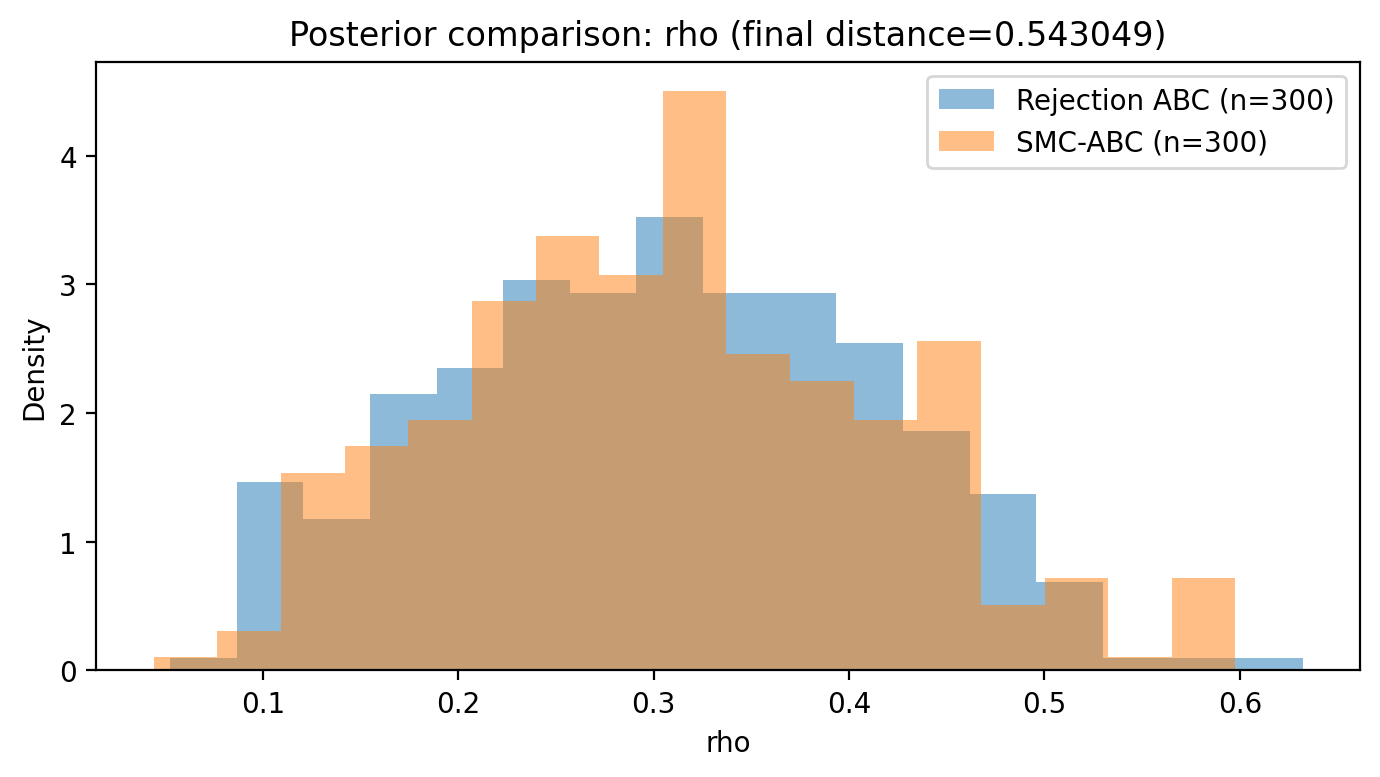
\includegraphics[width=\linewidth]{outputs/smc_abc/plots/rho_rejection_vs_smc_abc.png}
    \caption{$\rho$: rejection ABC versus SMC-ABC.}
\end{subfigure}
\hfill
\begin{subfigure}[t]{0.48\textwidth}
    \centering
    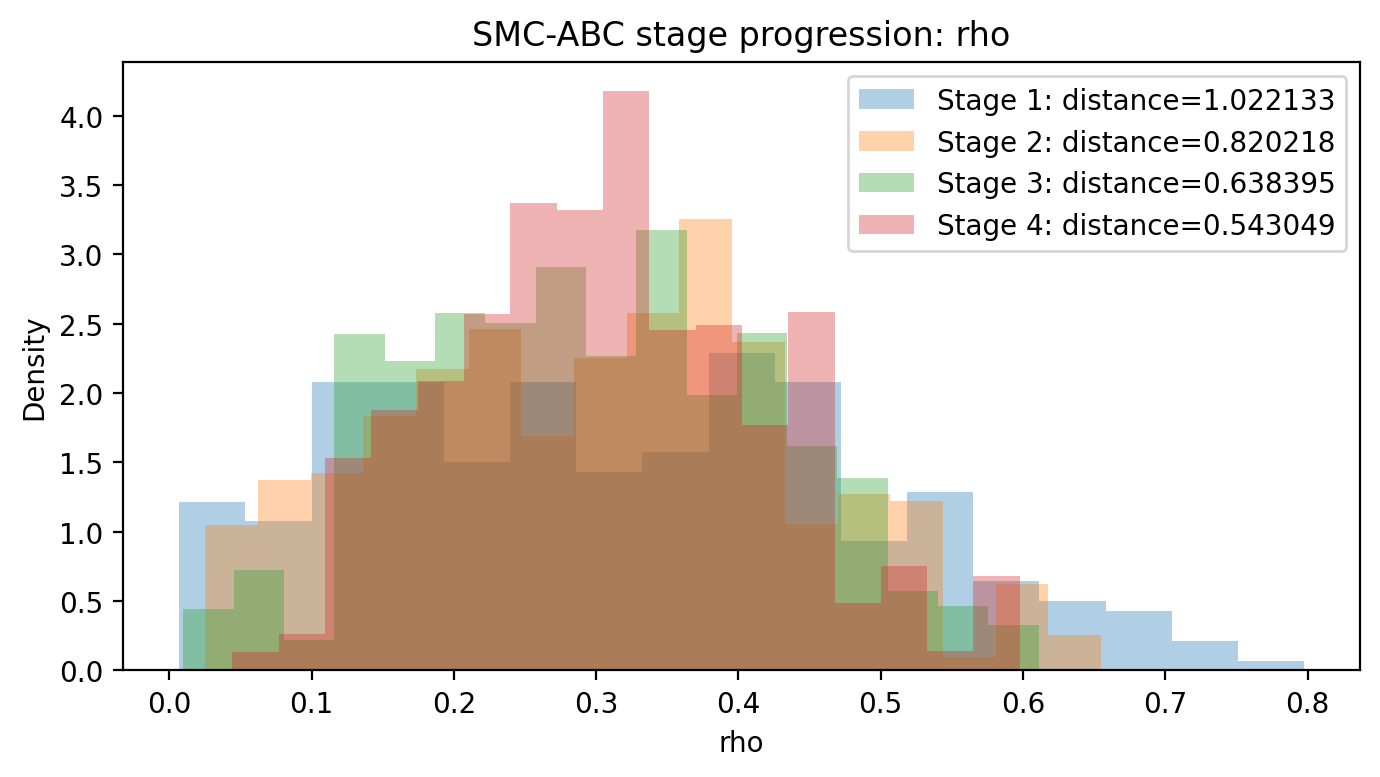
\includegraphics[width=\linewidth]{outputs/smc_abc/plots/rho_smc_abc_stage_progression.png}
    \caption{$\rho$: SMC-ABC stage progression.}
\end{subfigure}
\caption{Left column: posterior comparison between Reduced set I rejection ABC and SMC-ABC, plotted with matched sample counts. Right column: stage-by-stage posterior evolution in the SMC-ABC run.}
\label{fig:smc-results}
\end{figure}

Overall, the scripts and saved plots tell a coherent story after the upstream update to \texttt{abc\_rejection.py}. The baseline rejection ABC posterior is already informative, $\epsilon=0.01$ gives a reasonable balance between fit and sample size, Reduced set I is the preferred reduced-summary approximation to the rich-set posterior, regression adjustment shows that a looser threshold such as $\epsilon=0.05$ can still produce a nearly identical corrected posterior, and both ABC-MCMC and SMC-ABC confirm the same parameter conclusions while inheriting exactly the same Reduced set I calibration from the saved rejection reference file.

\appendix
\renewcommand{\thesection}{Appendix \Alph{section}}
\renewcommand{\thesubsection}{\Alph{section}.\arabic{subsection}}
\refstepcounter{section}
\phantomsection
\addcontentsline{toc}{section}{\thesection}
\section*{\thesection}
\label{app:supporting-material}

\subsection{Detailed Rejection-ABC Diagnostics}
\label{app:rejection-diagnostics}

This appendix collects the full rejection-ABC diagnostics that support Section~2. The main body keeps only the decisive points: $\epsilon=0.01$ is the working rejection threshold, Reduced set I is the preferred reduced-summary subset after the summary-statistic update, and all downstream extensions inherit that same calibration. The remaining figure gallery is kept here so that the report does not overload the main narrative with repetitive visual comparisons.

\subsubsection{Tolerance-choice diagnostics}

The first diagnostic question is why $\epsilon = 0.01$ was retained as the basic-ABC working tolerance. The detailed evidence comes from the eight summary overlays saved in \texttt{outputs/basic\_abc/sanity\_check/}, where the accepted simulated summaries for $\epsilon \in \{0.005,0.01,0.03\}$ are plotted against the observed value shown by the \textcolor{red}{red vertical line}.

For each panel, the \textcolor{red}{red vertical line} represents the calculated mean summary statistic from the observed data, namely
\[
\widehat{s}^{\,\mathrm{obs}}_j = \frac{1}{R}\sum_{r=1}^{R}\eta_j\!\left(Y^{(r)}\right),
\qquad R = 40.
\]
This is the same observed summary value used in the ABC distance calculation. Hence the diagnostic plots should be read as a comparison between the distribution of accepted simulated summaries and the empirical mean summary extracted from the observed replicates.

Across the eight summaries, the strictest tolerance $\epsilon = 0.005$ usually gives the tightest match to the observed summaries, but it uses only $500$ accepted draws and therefore produces visibly rougher histograms. At the other extreme, $\epsilon = 0.03$ yields $3000$ accepted draws, but this broader acceptance region admits many simulations whose summaries lie further from the observed line, resulting in posterior samples of higher variance. The intermediate choice $\epsilon = 0.01$ provides a better compromise: the accepted histograms remain centered near the observed summaries while still retaining $1000$ posterior draws for more stable inference.

Figures~\ref{fig:appendix-epsilon-diagnostics-1}--\ref{fig:appendix-epsilon-diagnostics-4} show the full set of diagnostic plots. For maximum infection fraction and time to peak, the overlays indicate that $\epsilon = 0.01$ retains a close match to the observed epidemic peak behavior while avoiding the extra spread seen at $\epsilon = 0.03$. For early infection growth, early rewiring growth, and degree variance, the same pattern holds, but the gain from moving from $\epsilon = 0.005$ to $\epsilon = 0.01$ is especially useful because the histogram becomes less noisy without a clear loss of fit.

The degree-variance, rewiring-per-infection, and peak-width diagnostics are particularly informative after the summary-statistic update. They show that the added network-adaptation and epidemic-width summaries are not arbitrary extras; they remain well aligned with the observed values at $\epsilon=0.01$ but become noticeably more diffuse at $\epsilon=0.03$. This is one of the clearest visual arguments for preferring $\epsilon = 0.01$ over both the noisier $\epsilon = 0.005$ fit and the more weakly targeted $\epsilon = 0.03$ fit.

\begin{figure}[H]
\centering
\begin{subfigure}[t]{0.49\textwidth}
    \centering
    
\includegraphics[width=\linewidth]{\detokenize{outputs/basic_abc/sanity_check/summary_Max infection fraction_overlay_eps_2026-04-12_23-11.png}}
    \caption{Maximum infection fraction diagnostic overlay.}
\end{subfigure}
\hfill
\begin{subfigure}[t]{0.49\textwidth}
    \centering
    
\includegraphics[width=\linewidth]{\detokenize{outputs/basic_abc/sanity_check/summary_Time to peak_overlay_eps_2026-04-12_23-11.png}}
    \caption{Time to peak diagnostic overlay.}
\end{subfigure}
\caption{First group of rejection-ABC sanity-check plots used to assess the tolerance choice.}
\label{fig:appendix-epsilon-diagnostics-1}
\end{figure}

\begin{figure}[H]
\centering
\begin{subfigure}[t]{0.49\textwidth}
    \centering
    
\includegraphics[width=\linewidth]{\detokenize{outputs/basic_abc/sanity_check/summary_Early growth rate of infection_overlay_eps_2026-04-12_23-11.png}}
    \caption{Early infection growth diagnostic overlay.}
\end{subfigure}
\hfill
\begin{subfigure}[t]{0.49\textwidth}
    \centering
    
\includegraphics[width=\linewidth]{\detokenize{outputs/basic_abc/sanity_check/summary_Early growth rate of rewiring_overlay_eps_2026-04-12_23-11.png}}
    \caption{Early rewiring growth diagnostic overlay.}
\end{subfigure}
\caption{Second group of rejection-ABC sanity-check plots used to assess the tolerance choice.}
\label{fig:appendix-epsilon-diagnostics-2}
\end{figure}

\begin{figure}[H]
\centering
\begin{subfigure}[t]{0.49\textwidth}
    \centering
    
\includegraphics[width=\linewidth]{\detokenize{outputs/basic_abc/sanity_check/summary_Variance structure of degree counts_overlay_eps_2026-04-12_23-11.png}}
    \caption{Degree-variance diagnostic overlay.}
\end{subfigure}
\hfill
\begin{subfigure}[t]{0.49\textwidth}
    \centering
    
\includegraphics[width=\linewidth]{\detokenize{outputs/basic_abc/sanity_check/summary_Late decay rate of infection_overlay_eps_2026-04-12_23-11.png}}
    \caption{Late infection decay diagnostic overlay.}
\end{subfigure}
\caption{Third group of rejection-ABC sanity-check plots used to assess the tolerance choice.}
\label{fig:appendix-epsilon-diagnostics-3}
\end{figure}

\begin{figure}[H]
\centering
\begin{subfigure}[t]{0.49\textwidth}
    \centering
    
\includegraphics[width=\linewidth]{\detokenize{outputs/basic_abc/sanity_check/summary_Rewiring per infection_overlay_eps_2026-04-12_23-11.png}}
    \caption{Rewiring-per-infection diagnostic overlay.}
\end{subfigure}
\hfill
\begin{subfigure}[t]{0.49\textwidth}
    \centering
    
\includegraphics[width=\linewidth]{\detokenize{outputs/basic_abc/sanity_check/summary_Infection peak width at half maximum_overlay_eps_2026-04-12_23-11.png}}
    \caption{Peak-width-at-half-maximum diagnostic overlay.}
\end{subfigure}
\caption{Fourth group of rejection-ABC sanity-check plots used to assess the tolerance choice.}
\label{fig:appendix-epsilon-diagnostics-4}
\end{figure}

\subsubsection{Full summary-set comparison gallery}

The next question is how the reduced-summary comparison changed once rewiring per infection and peak width were added to the full summary set. The main text already gave the decisive answer: Reduced set I became the preferred reduced summary because it stayed visually close to the rich-set posterior while also attaining the smallest normalized posterior spread in the heatmap. Figures~\ref{fig:appendix-summary-comparisons-1}--\ref{fig:appendix-summary-comparisons-5} collect the full rich-set versus reduced-set gallery for sets A--I at $\epsilon = 0.01$.

Two points are worth noting. First, the old Reduced set E remains competitive, but it is no longer the natural endpoint once the two new summaries are introduced. Second, the new sets G, H, and I are the relevant competitors after the update because they explicitly incorporate rewiring per infection, and set I further adds the epidemic peak-width statistic. Visually, that extra peak-width information is what makes Reduced set I the most faithful low-dimensional approximation to the updated rich-set posterior.

\begin{figure}[H]
\centering
\begin{subfigure}[t]{0.49\textwidth}
    \centering
    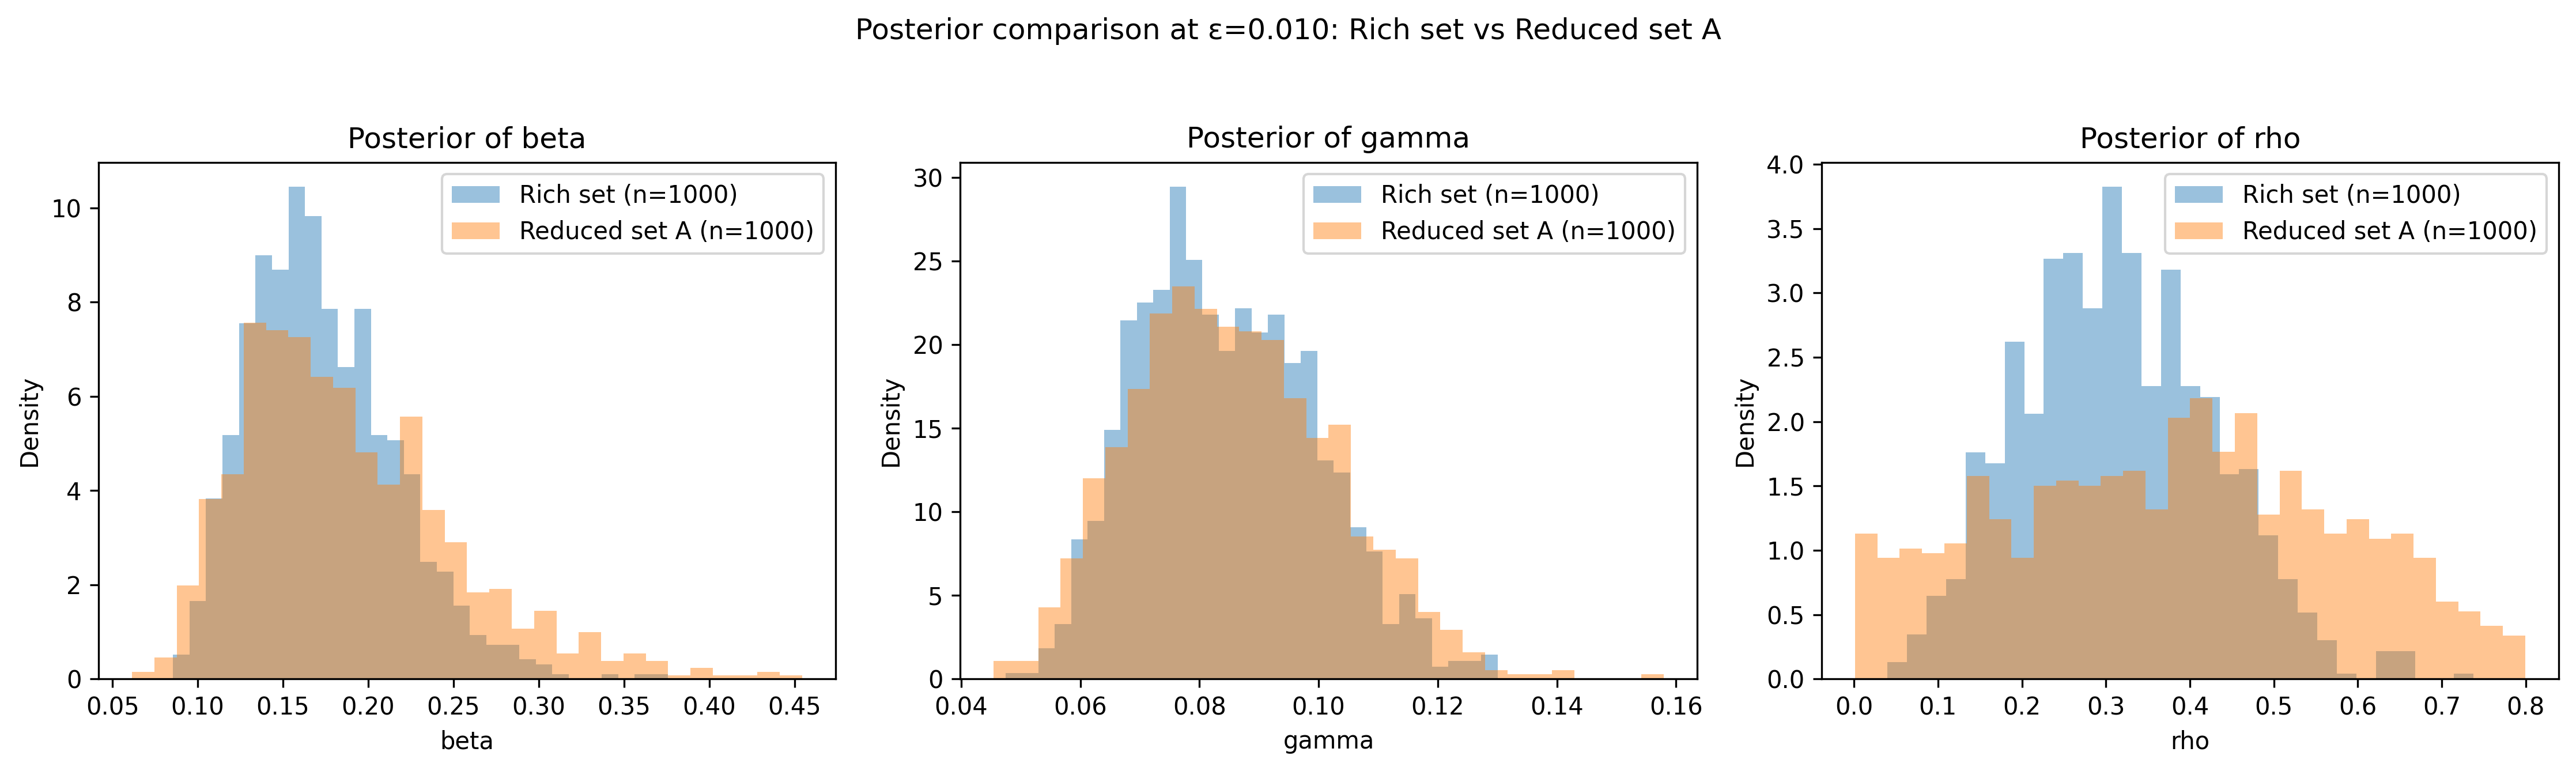
\includegraphics[width=\linewidth]{outputs/basic_abc/summary_set_study/posterior_rich_set_vs_reduced_set_a_eps-0.0100_2026-04-12_23-11.png}
    \caption{Rich set versus Reduced set A.}
\end{subfigure}
\hfill
\begin{subfigure}[t]{0.49\textwidth}
    \centering
    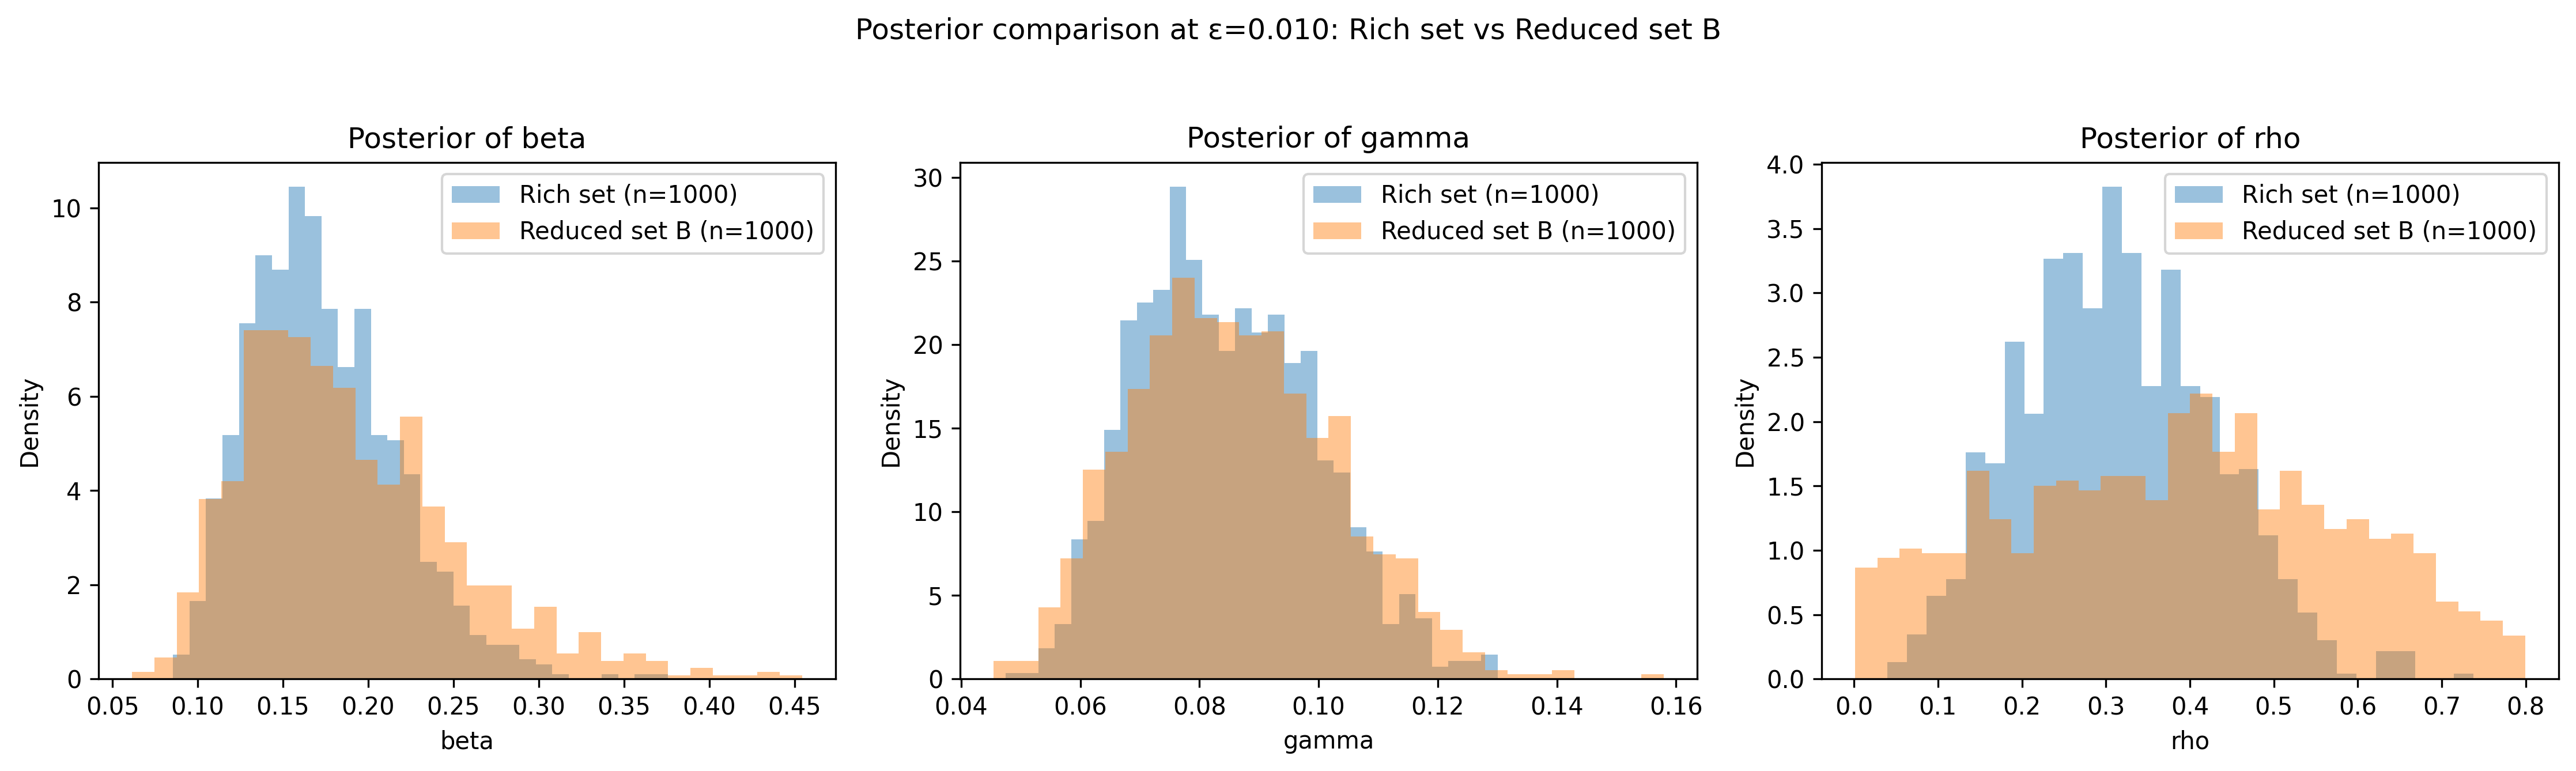
\includegraphics[width=\linewidth]{outputs/basic_abc/summary_set_study/posterior_rich_set_vs_reduced_set_b_eps-0.0100_2026-04-12_23-11.png}
    \caption{Rich set versus Reduced set B.}
\end{subfigure}
\caption{First group of rich-set versus reduced-set posterior comparisons at $\epsilon = 0.01$.}
\label{fig:appendix-summary-comparisons-1}
\end{figure}

\begin{figure}[H]
\centering
\begin{subfigure}[t]{0.49\textwidth}
    \centering
    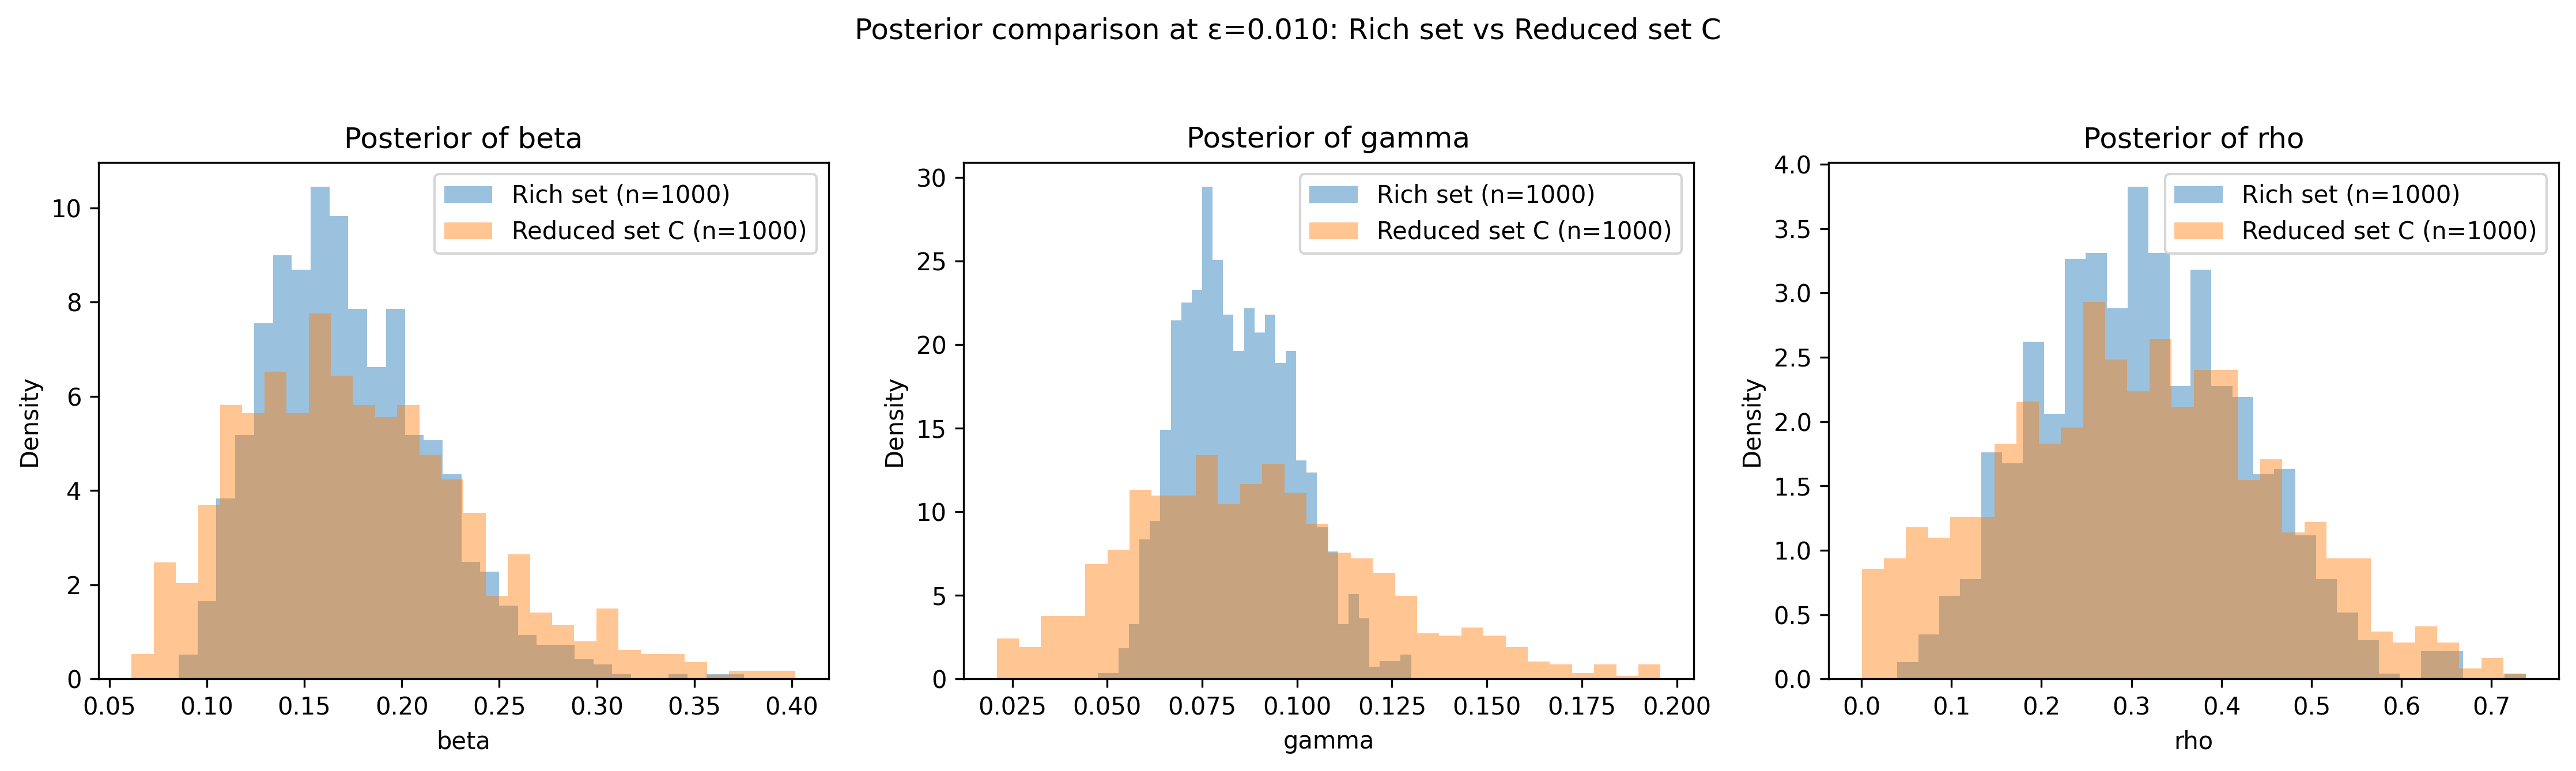
\includegraphics[width=\linewidth]{outputs/basic_abc/summary_set_study/posterior_rich_set_vs_reduced_set_c_eps-0.0100_2026-04-12_23-11.png}
    \caption{Rich set versus Reduced set C.}
\end{subfigure}
\hfill
\begin{subfigure}[t]{0.49\textwidth}
    \centering
    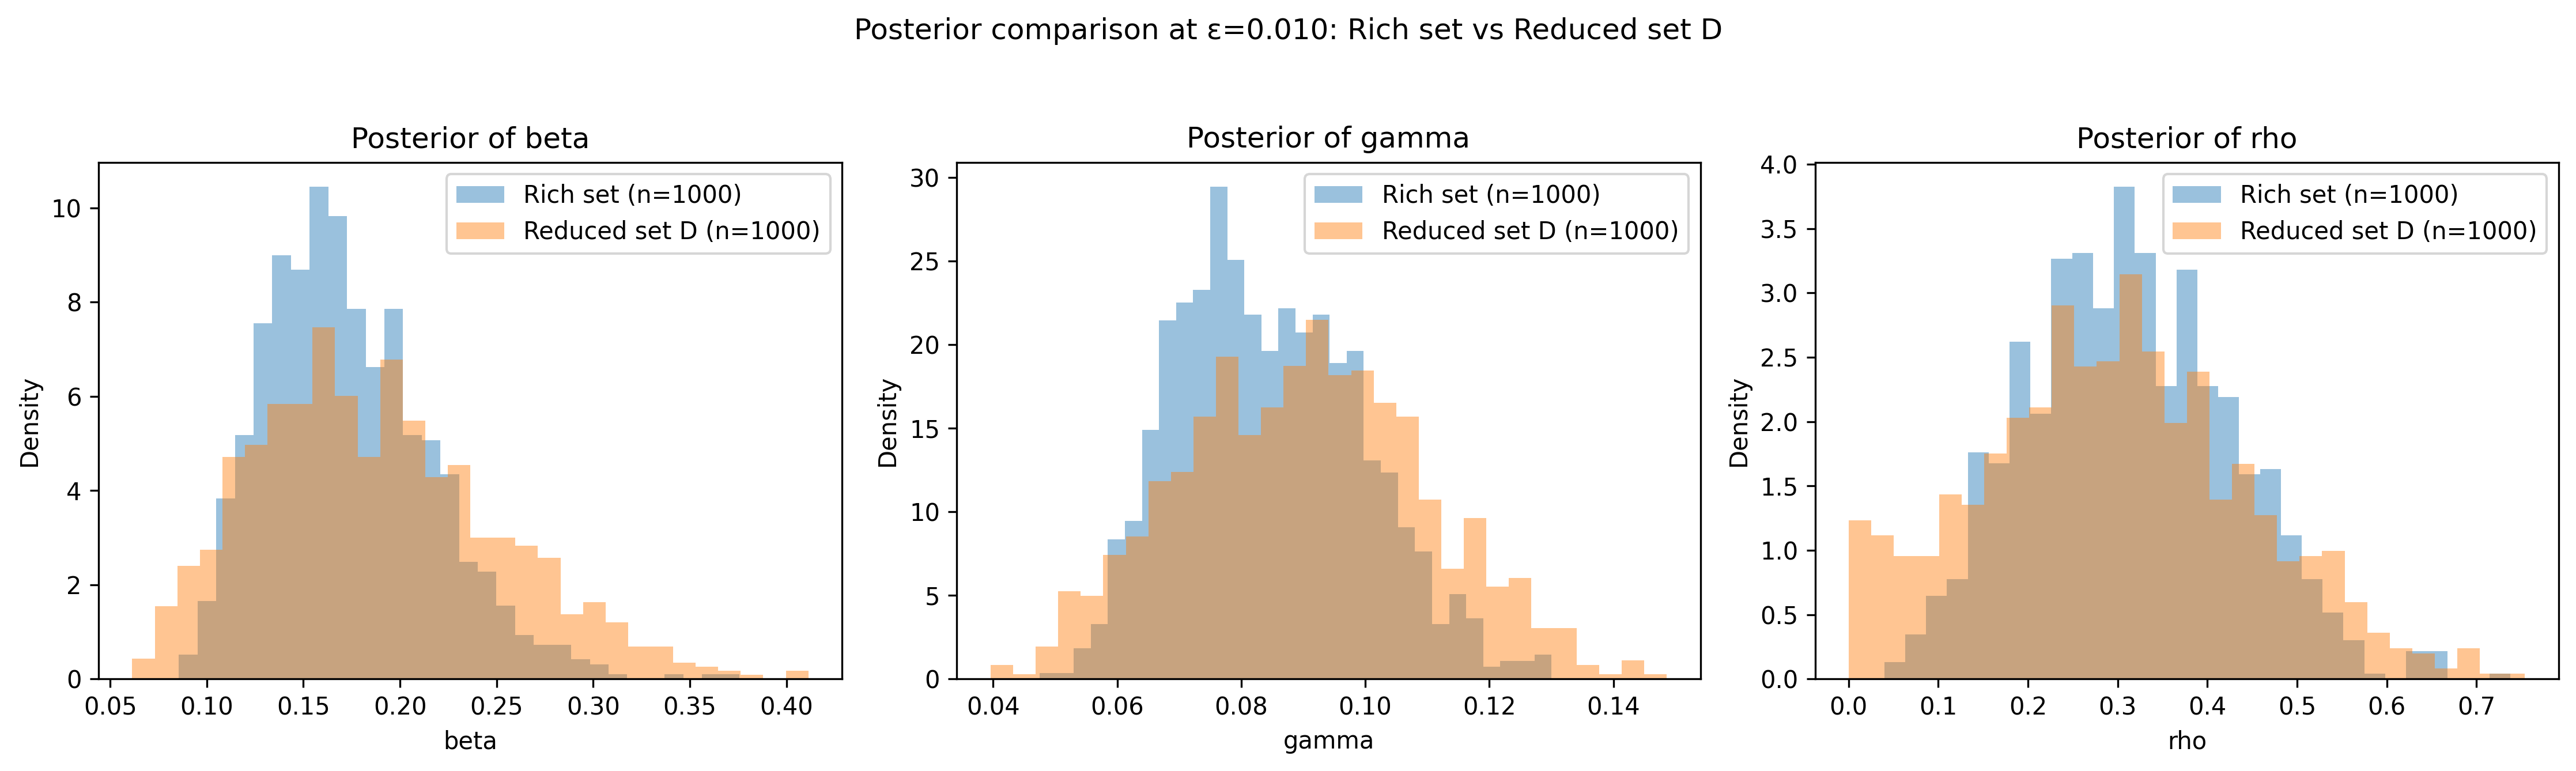
\includegraphics[width=\linewidth]{outputs/basic_abc/summary_set_study/posterior_rich_set_vs_reduced_set_d_eps-0.0100_2026-04-12_23-11.png}
    \caption{Rich set versus Reduced set D.}
\end{subfigure}
\caption{Second group of rich-set versus reduced-set posterior comparisons at $\epsilon = 0.01$.}
\label{fig:appendix-summary-comparisons-2}
\end{figure}

\begin{figure}[H]
\centering
\begin{subfigure}[t]{0.49\textwidth}
    \centering
    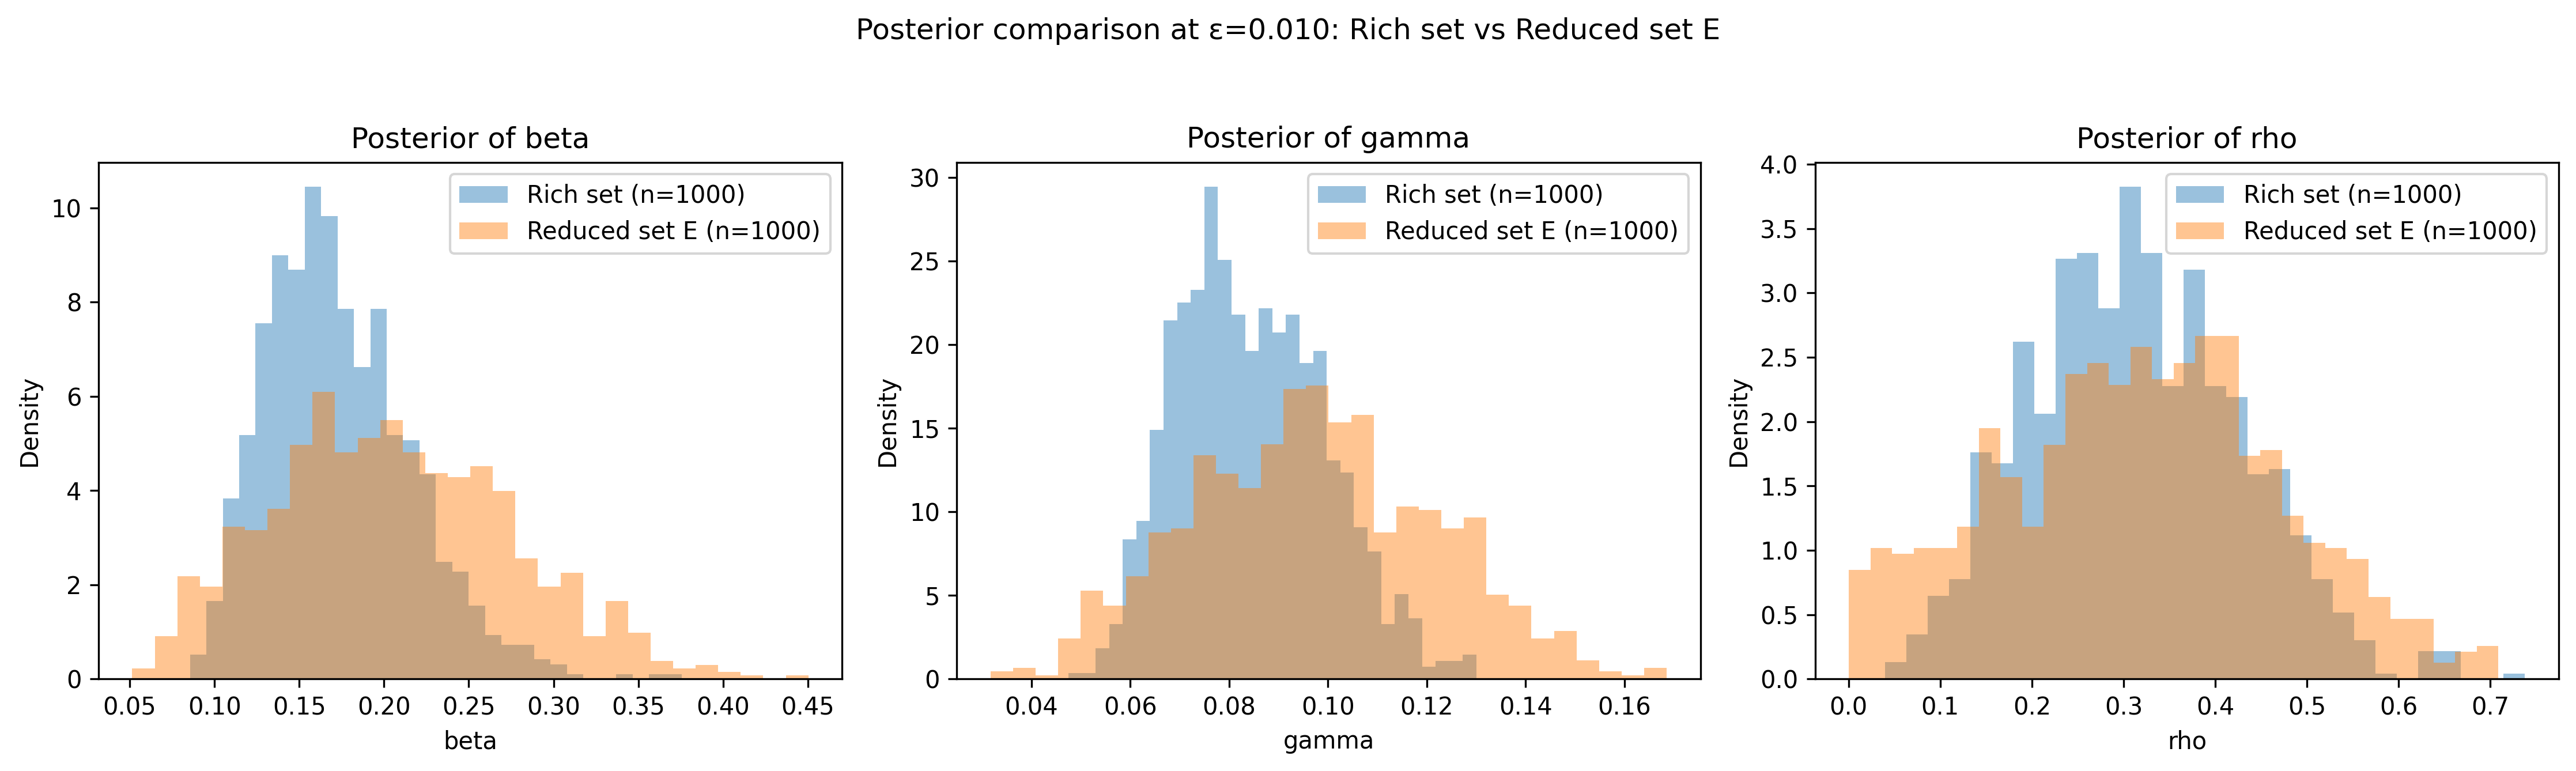
\includegraphics[width=\linewidth]{outputs/basic_abc/summary_set_study/posterior_rich_set_vs_reduced_set_e_eps-0.0100_2026-04-12_23-11.png}
    \caption{Rich set versus Reduced set E.}
\end{subfigure}
\hfill
\begin{subfigure}[t]{0.49\textwidth}
    \centering
    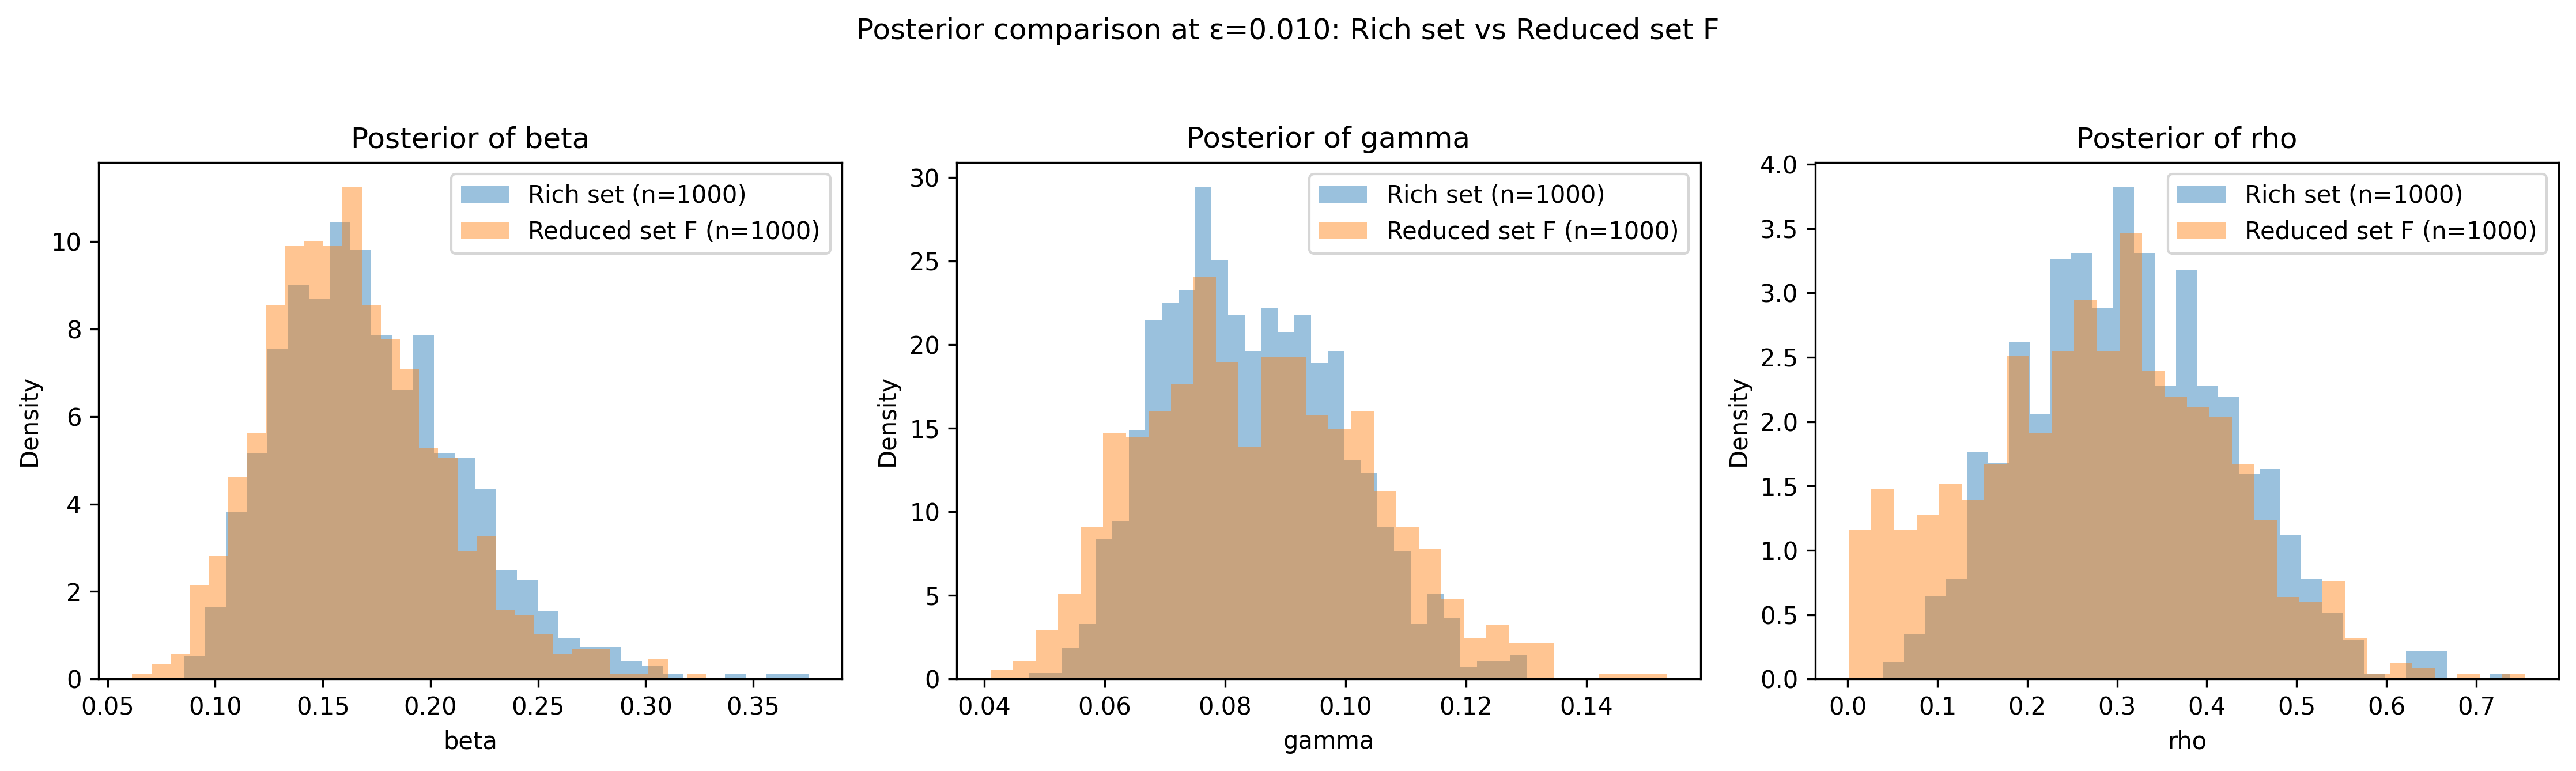
\includegraphics[width=\linewidth]{outputs/basic_abc/summary_set_study/posterior_rich_set_vs_reduced_set_f_eps-0.0100_2026-04-12_23-11.png}
    \caption{Rich set versus Reduced set F.}
\end{subfigure}
\caption{Third group of rich-set versus reduced-set posterior comparisons at $\epsilon = 0.01$.}
\label{fig:appendix-summary-comparisons-3}
\end{figure}

\begin{figure}[H]
\centering
\begin{subfigure}[t]{0.49\textwidth}
    \centering
    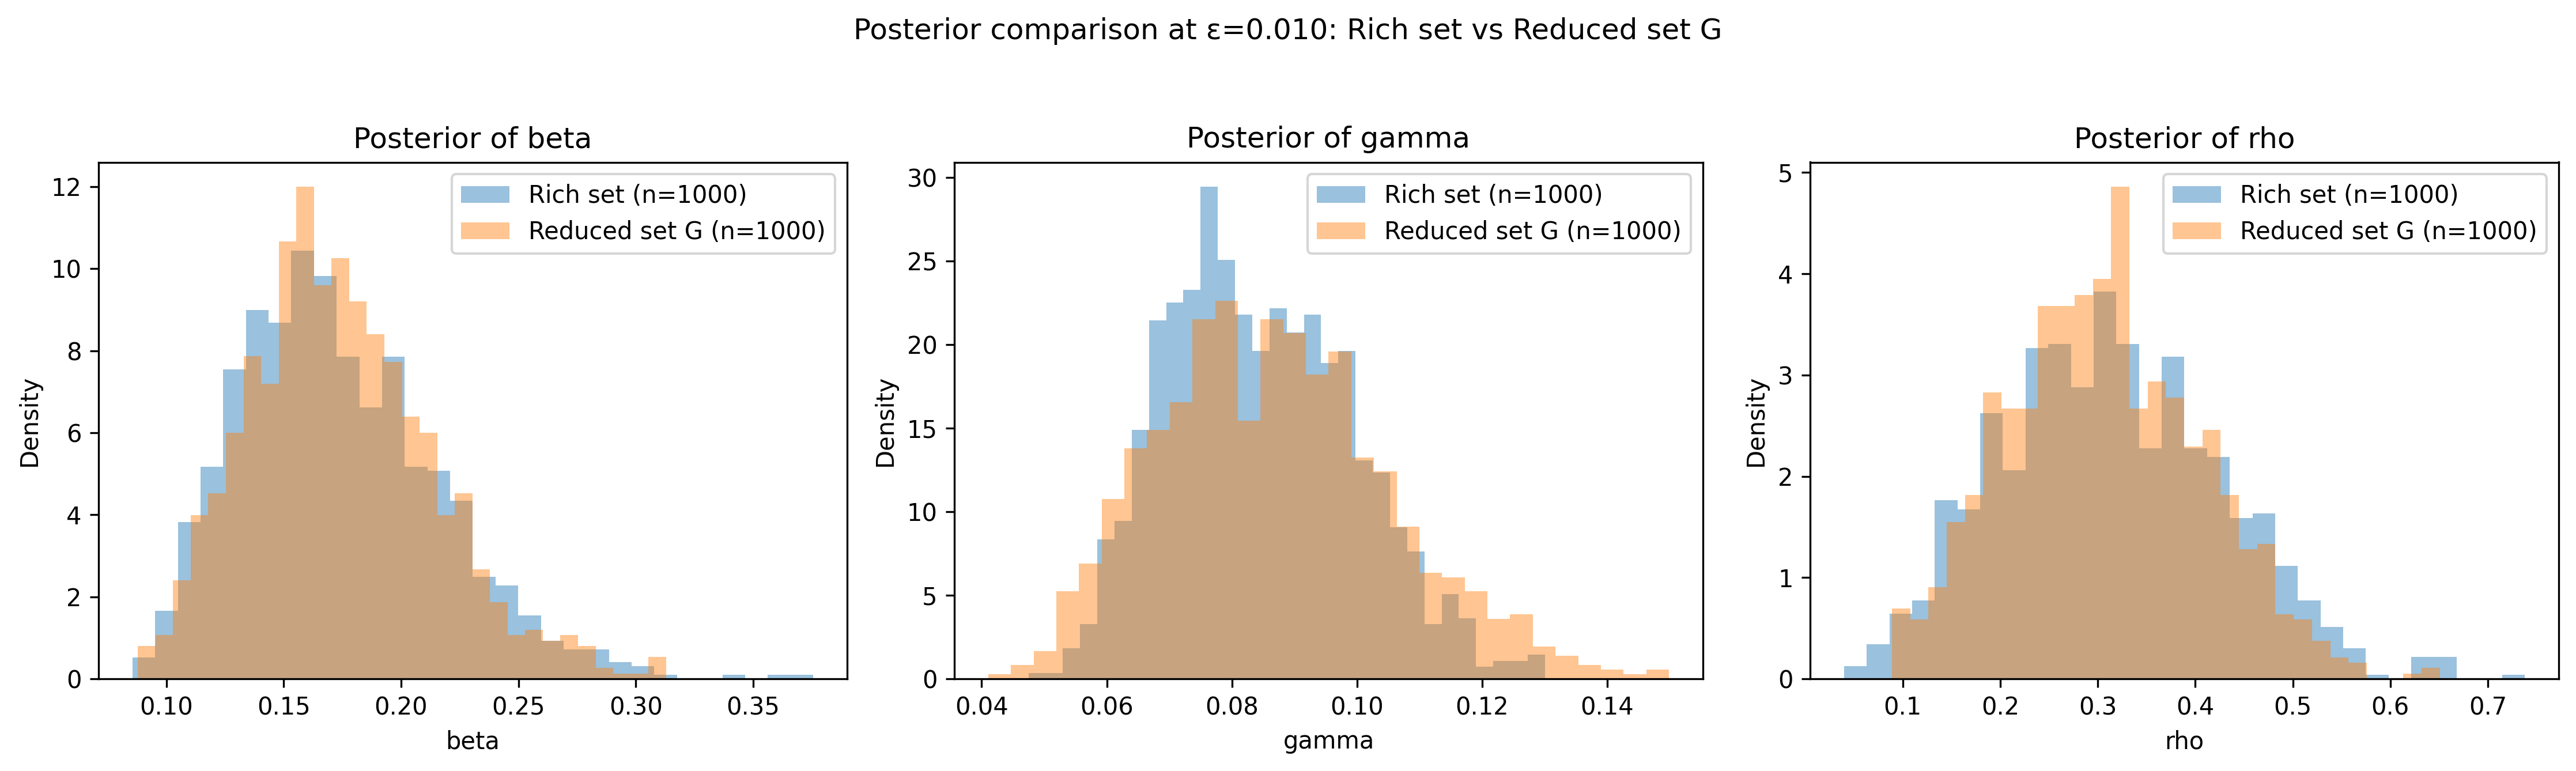
\includegraphics[width=\linewidth]{outputs/basic_abc/summary_set_study/posterior_rich_set_vs_reduced_set_g_eps-0.0100_2026-04-12_23-11.png}
    \caption{Rich set versus Reduced set G.}
\end{subfigure}
\hfill
\begin{subfigure}[t]{0.49\textwidth}
    \centering
    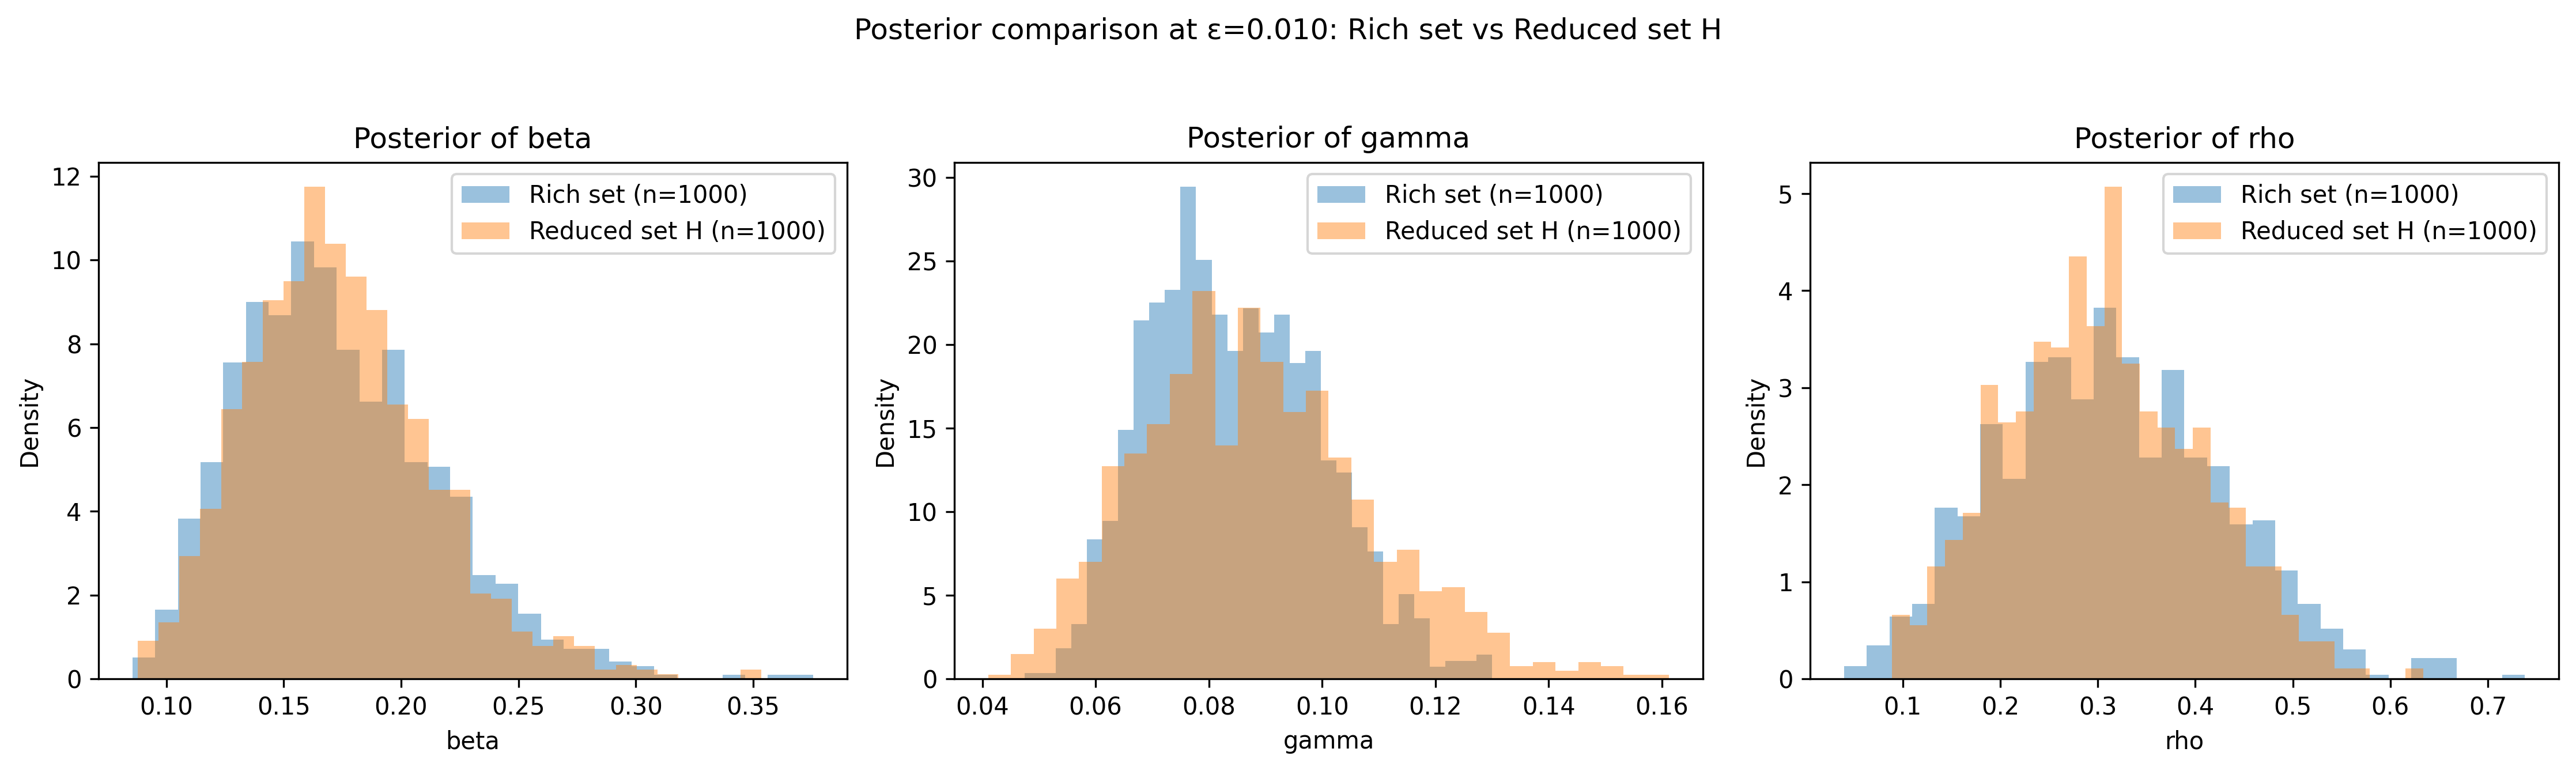
\includegraphics[width=\linewidth]{outputs/basic_abc/summary_set_study/posterior_rich_set_vs_reduced_set_h_eps-0.0100_2026-04-12_23-11.png}
    \caption{Rich set versus Reduced set H.}
\end{subfigure}
\caption{Fourth group of rich-set versus reduced-set posterior comparisons at $\epsilon = 0.01$.}
\label{fig:appendix-summary-comparisons-4}
\end{figure}

\begin{figure}[H]
\centering
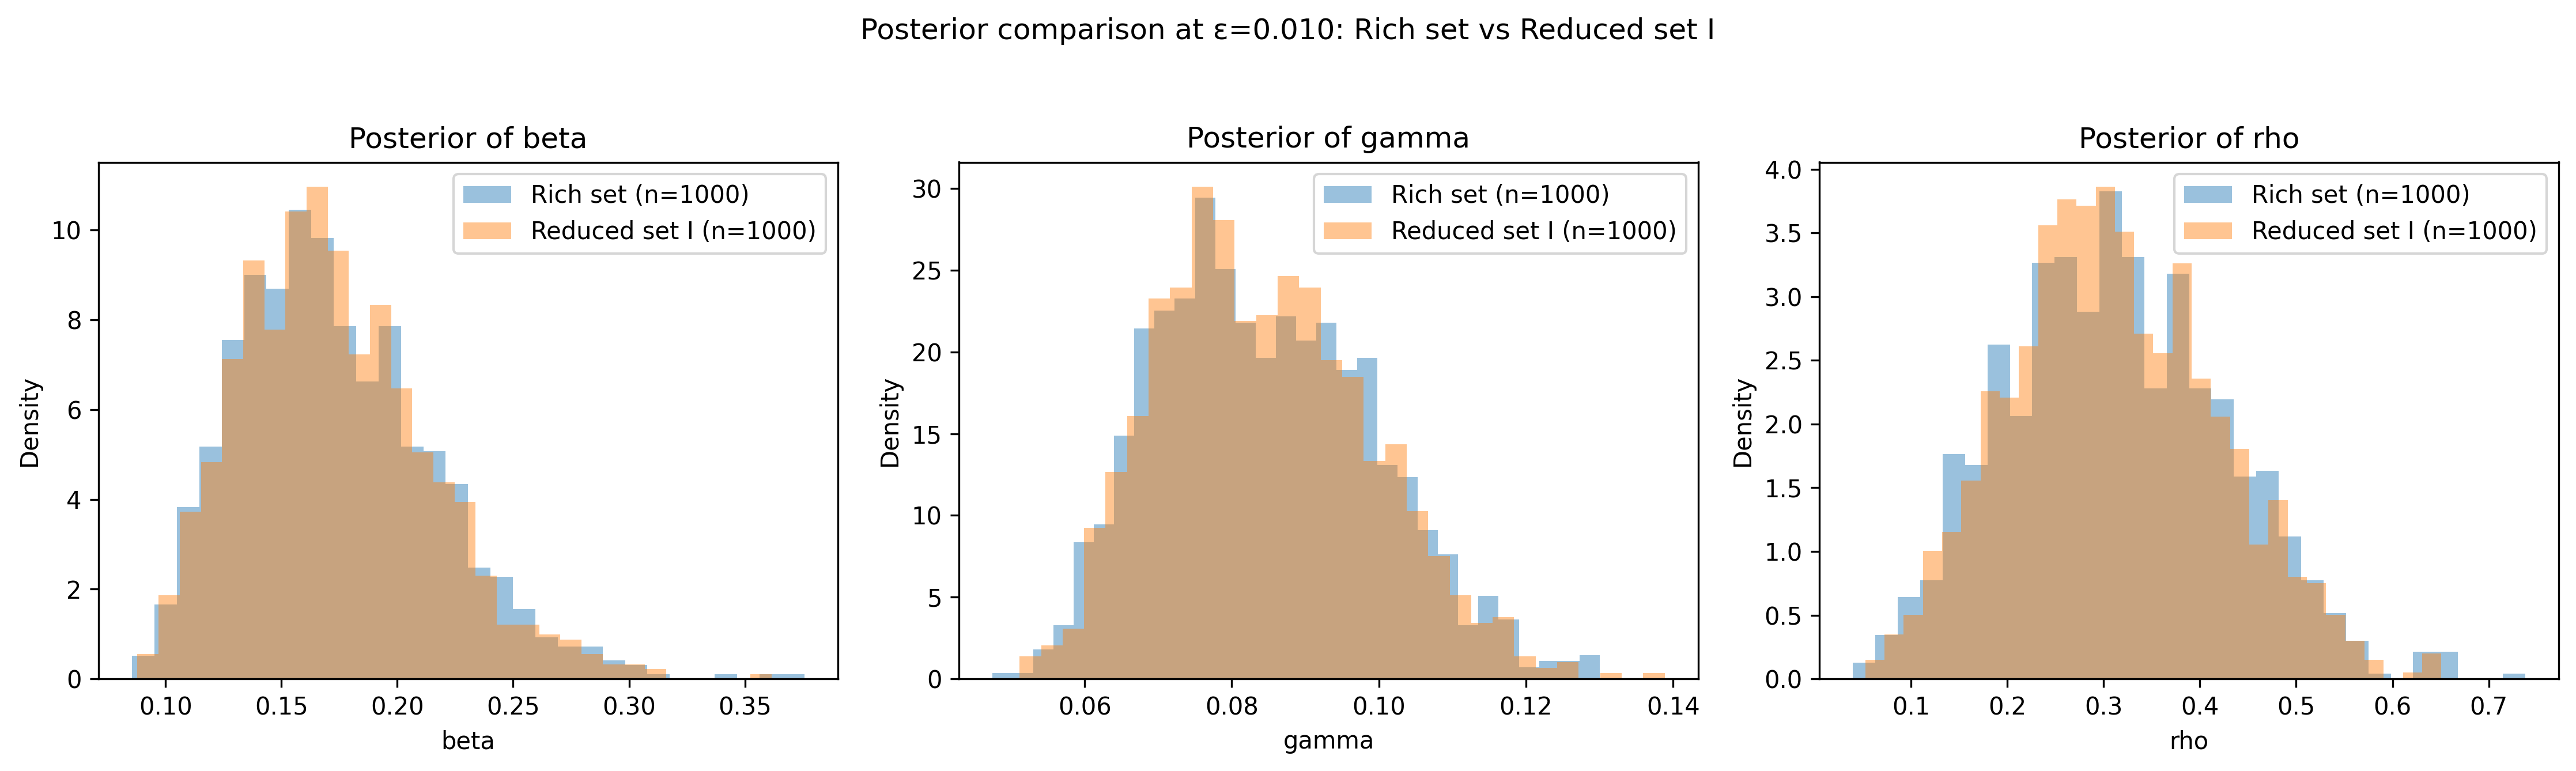
\includegraphics[width=0.58\textwidth]{outputs/basic_abc/summary_set_study/posterior_rich_set_vs_reduced_set_i_eps-0.0100_2026-04-12_23-11.png}
\caption{Final rich-set versus reduced-set comparison at $\epsilon = 0.01$: Reduced set I.}
\label{fig:appendix-summary-comparisons-5}
\end{figure}

\begin{thebibliography}{}

\bibitem[Beaumont et~al.(2002)Beaumont, Zhang, and Balding]{beaumont2002}
Beaumont, Mark~A., Wenyang Zhang, and David~J. Balding. 2002.
``Approximate Bayesian Computation in Population Genetics.''
\emph{Genetics} 162 (4): 2025--2035.

\bibitem[Marjoram et~al.(2003)Marjoram, Molitor, Plagnol, and Tavar\'e]{marjoram2003}
Marjoram, Paul, John Molitor, Vincent Plagnol, and Simon Tavar\'e. 2003.
``Markov Chain Monte Carlo Without Likelihoods.''
\emph{Proceedings of the National Academy of Sciences} 100 (26): 15324--15328.

\end{thebibliography}

\end{document}
